\documentclass[preprint,12pt,authoryear]{elsarticle}
\usepackage[utf8]{inputenc}
\usepackage[margin=2cm]{geometry}
\usepackage{graphicx}
\usepackage{multirow}
\usepackage{amssymb}
\usepackage{amsmath}
\usepackage{setspace}
\usepackage{outlines}
\usepackage{enumitem}
\usepackage{xcolor}
\usepackage{upgreek}
\usepackage{mathabx}
\usepackage{algorithm}
\usepackage{algorithmic}
\usepackage{amsthm}
\usepackage[labelfont=bf,font=small]{caption}
\usepackage{epsfig}
\usepackage{geometry}
\usepackage{subfigure}
\usepackage[textsize=tiny]{todonotes}
\usepackage[normalem]{ulem}
\usepackage{lipsum}
\usepackage{array}
\usepackage{booktabs}
\usepackage{lineno}
\usepackage{array}
\usepackage{tikz}
\usepackage[english]{babel}
\usepackage{animate}
\usepackage{cancel}

\usepackage[]{siunitx}
\sisetup{range-units=single,separate-uncertainty = true,print-unity-mantissa=false,per-mode=symbol,range-phrase = \text{--},
inter-unit-product=\cdot
}

\usepackage[
    protrusion=true,
    activate={true,nocompatibility},
    final,
    tracking=true,
    kerning=true,
    spacing=true,
    factor=1100]{microtype}
    
\SetTracking{encoding={*}, shape=sc}{40}

\usepackage{outlines}
\usepackage{enumitem}

\definecolor{lightblue}{rgb}{0.63, 0.74, 0.78}
\definecolor{seagreen}{rgb}{0.18, 0.42, 0.41}
\definecolor{orange}{rgb}{0.85, 0.55, 0.13}
\definecolor{silver}{rgb}{0.69, 0.67, 0.66}
\definecolor{rust}{rgb}{0.72, 0.26, 0.06}
\definecolor{purp}{RGB}{68, 14, 156}

\definecolor{zblue}{RGB}{8,81,156}
\definecolor{zpurp}{RGB}{84,39,143}
\definecolor{zred}{RGB}{165,15,21}

\colorlet{lightrust}{rust!50!white}
\colorlet{lightorange}{orange!25!white}
\colorlet{lightlightblue}{lightblue}
\colorlet{lightsilver}{silver!30!white}
\colorlet{darkorange}{orange!75!black}
\colorlet{darksilver}{silver!65!black}
\colorlet{darklightblue}{lightblue!65!black}
\colorlet{darkrust}{rust!85!black}
\colorlet{darkseagreen}{seagreen!85!black}



\usepackage{hyperref}
\hypersetup{
  colorlinks=true,
}
\usepackage{tabularx}
\usepackage{bbm}
\usepackage{bm}

\usepackage[nameinlink]{cleveref}
\crefname{equation}{}{}
\def\appendixname{}
\crefname{appendix}{}{}


\usepackage{setspace}
% \doublespacing
\setlength{\heavyrulewidth}{1.5pt}
% \setlength{\abovetopsep}{4pt}
 
\usepackage{soul}
\sethlcolor{yellow}

\usepackage[parfill]{parskip}

\usepackage{lineno}
\usepackage{tcolorbox}
%\linenumbers

%% Self-defined Macros
\newcommand{\bn}[1]{\mathbf{#1}}
\newcommand{\bs}[1]{\ensuremath{\boldsymbol{#1}}}
\newcommand{\mc}[1]{\ensuremath{\mathcal{#1}}}
\newcommand{\norm}[1]{\ensuremath \lVert #1 \rVert}
\newcommand{\GD}[1]{ D #1 (\boldsymbol{F})[\boldsymbol{H}]}
\newcommand{\GDI}[1]{ D #1 (\boldsymbol{I})[\boldsymbol{H}]}
\newcommand{\Lin}[1]{ L_{\boldsymbol{F}} #1 [\boldsymbol{H}]}
\newcommand{\LinI}[1]{ L_{\boldsymbol{I}} #1 [\boldsymbol{H}]}
\newcommand{\Dm}[1]{\ensuremath{\boldsymbol{\varphi} } }
\newcommand{\tr}[1]{\textcolor{red}{#1}}
\newcommand{\ignore}[1]{}
\newcommand{\fracp}[2]{\frac{\partial #1}{\partial #2}}
\newcommand{\wt}[1]{\widetilde{#1}}
\renewcommand{\[}{\left[}
\renewcommand{\]}{\right]}
\renewcommand{\(}{\left(}
\renewcommand{\)}{\right)}
\newcommand{\tn}{\textnormal}
\newcommand{\gradX}{\nabla_{\bm{X}}}
\newcommand{\gradx}{\nabla_{\bm{x}}}
\newcommand{\gradF}{\nabla_{\bn{F}}}

%\newcommant{\pfrac[2]}{\frac{\partial {#1}}{\partial {#2}}}

%% Coloring for comments
\usepackage{color,tikz,soul}
\newcommand{\jbe}[1]{\textcolor{violet}{#1}}

\newcommand{\rev}[1]{\textcolor{red}{#1}}

\usepackage{xcolor, soul}
\sethlcolor{yellow}
\usepackage[per-mode=symbol]{siunitx}

\setlength{\tabcolsep}{12pt}

\renewcommand{\thetable}{\arabic{table}} % Originally Roman uppercase

\journal{ME517---Mechanics of Soft Materials}
\setlength{\marginparwidth}{2cm}
\begin{document}

% \documentclass[preprint,12pt,authoryear]{elsarticle}
% \usepackage[utf8]{inputenc}
\usepackage[margin=2cm]{geometry}
\usepackage{graphicx}
\usepackage{multirow}
\usepackage{amssymb}
\usepackage{amsmath}
\usepackage{setspace}
\usepackage{outlines}
\usepackage{enumitem}
\usepackage{xcolor}
\usepackage{upgreek}
\usepackage{mathabx}
\usepackage{algorithm}
\usepackage{algorithmic}
\usepackage{amsthm}
\usepackage[labelfont=bf,font=small]{caption}
\usepackage{epsfig}
\usepackage{geometry}
\usepackage{subfigure}
\usepackage[textsize=tiny]{todonotes}
\usepackage[normalem]{ulem}
\usepackage{lipsum}
\usepackage{array}
\usepackage{booktabs}
\usepackage{lineno}
\usepackage{array}
\usepackage{tikz}
\usepackage[english]{babel}
\usepackage{animate}
\usepackage{cancel}

\usepackage[]{siunitx}
\sisetup{range-units=single,separate-uncertainty = true,print-unity-mantissa=false,per-mode=symbol,range-phrase = \text{--},
inter-unit-product=\cdot
}

\usepackage[
    protrusion=true,
    activate={true,nocompatibility},
    final,
    tracking=true,
    kerning=true,
    spacing=true,
    factor=1100]{microtype}
    
\SetTracking{encoding={*}, shape=sc}{40}

\usepackage{outlines}
\usepackage{enumitem}

\definecolor{lightblue}{rgb}{0.63, 0.74, 0.78}
\definecolor{seagreen}{rgb}{0.18, 0.42, 0.41}
\definecolor{orange}{rgb}{0.85, 0.55, 0.13}
\definecolor{silver}{rgb}{0.69, 0.67, 0.66}
\definecolor{rust}{rgb}{0.72, 0.26, 0.06}
\definecolor{purp}{RGB}{68, 14, 156}

\definecolor{zblue}{RGB}{8,81,156}
\definecolor{zpurp}{RGB}{84,39,143}
\definecolor{zred}{RGB}{165,15,21}

\colorlet{lightrust}{rust!50!white}
\colorlet{lightorange}{orange!25!white}
\colorlet{lightlightblue}{lightblue}
\colorlet{lightsilver}{silver!30!white}
\colorlet{darkorange}{orange!75!black}
\colorlet{darksilver}{silver!65!black}
\colorlet{darklightblue}{lightblue!65!black}
\colorlet{darkrust}{rust!85!black}
\colorlet{darkseagreen}{seagreen!85!black}



\usepackage{hyperref}
\hypersetup{
  colorlinks=true,
}
\usepackage{tabularx}
\usepackage{bbm}
\usepackage{bm}

\usepackage[nameinlink]{cleveref}
\crefname{equation}{}{}
\def\appendixname{}
\crefname{appendix}{}{}


\usepackage{setspace}
% \doublespacing
\setlength{\heavyrulewidth}{1.5pt}
% \setlength{\abovetopsep}{4pt}
 
\usepackage{soul}
\sethlcolor{yellow}

\usepackage[parfill]{parskip}

\usepackage{lineno}
\usepackage{tcolorbox}
%\linenumbers

% %% Self-defined Macros
\newcommand{\bn}[1]{\mathbf{#1}}
\newcommand{\bs}[1]{\ensuremath{\boldsymbol{#1}}}
\newcommand{\mc}[1]{\ensuremath{\mathcal{#1}}}
\newcommand{\norm}[1]{\ensuremath \lVert #1 \rVert}
\newcommand{\GD}[1]{ D #1 (\boldsymbol{F})[\boldsymbol{H}]}
\newcommand{\GDI}[1]{ D #1 (\boldsymbol{I})[\boldsymbol{H}]}
\newcommand{\Lin}[1]{ L_{\boldsymbol{F}} #1 [\boldsymbol{H}]}
\newcommand{\LinI}[1]{ L_{\boldsymbol{I}} #1 [\boldsymbol{H}]}
\newcommand{\Dm}[1]{\ensuremath{\boldsymbol{\varphi} } }
\newcommand{\tr}[1]{\textcolor{red}{#1}}
\newcommand{\ignore}[1]{}
\newcommand{\fracp}[2]{\frac{\partial #1}{\partial #2}}
\newcommand{\wt}[1]{\widetilde{#1}}
\renewcommand{\[}{\left[}
\renewcommand{\]}{\right]}
\renewcommand{\(}{\left(}
\renewcommand{\)}{\right)}
\newcommand{\tn}{\textnormal}
\newcommand{\gradX}{\nabla_{\bm{X}}}
\newcommand{\gradx}{\nabla_{\bm{x}}}
\newcommand{\gradF}{\nabla_{\bn{F}}}

%\newcommant{\pfrac[2]}{\frac{\partial {#1}}{\partial {#2}}}

%% Coloring for comments
\usepackage{color,tikz,soul}
\newcommand{\jbe}[1]{\textcolor{violet}{#1}}

\newcommand{\rev}[1]{\textcolor{red}{#1}}

\usepackage{xcolor, soul}
\sethlcolor{yellow}
\usepackage[per-mode=symbol]{siunitx}

\setlength{\tabcolsep}{12pt}

\renewcommand{\thetable}{\arabic{table}} % Originally Roman uppercase

% \journal{ME517---Mechanics of Soft Materials}
% \setlength{\marginparwidth}{2cm}
% \newcommand\C[1]\null %\C{for inline comments}
% \begin{document}

% \section*{Project II: Literature Review (due Oct 3)}

The second step in your semester-long research proposal development is to contextualize your problem within the current field of your choice, demonstrate your understanding of the state-of-the-art, and identify something we don't yet understand but need to---this is the gap your (hypothetical) proposed project would seek to fill.

You'll execute this portion of the project as an outline. 
This outline does not need to be long! 
It does, however, need to be very clear, as you'll be expanding on it later. 
The sections should be the following:

\renewcommand{\outlinei}{enumerate}
\renewcommand{\outlineii}{itemize}
\begin{outline}
    \1 \textbf{Introductory context}
        \2 Add one or two bullet points briefly framing the history of your topic and its significance. 
        \2 Citations here are important---there should be several well-placed citations in each of these bullet points, and good review papers are especially helpful to lean on for context. 
        \2 \textit{\textbf{Example}: While gradient materials occur widely in nature---the structurally protective gradient of squid beaks [1], junctions between ligaments and bones [2], and the byssus threads that hold mussels to rocks [3] to name a few---polymeric gradient materials were only first considered in an engineering context in 1972 [4].}
    \1 \textbf{The state of the field}
        \2 In one or two bullet points, explain how things are done in the area of your project at the present moment. 
        \2 This can include any of experimentation, computational methods, and/or theory.
        \2 \textit{\textbf{Example 1}: Compositional gradients in engineered materials are typically produced in one of three ways: spatially (1) varying polymer crosslink density, e.g. using ultraviolet light-sensitive reactive groups [5, 6], (2) seeding of micro- or nanoparticles using centrifugation [7], electric fields [8], or other methods [9], or (3) using porosity to create structural gradients using dissolvable template-making materials [10].}
        \2 \textit{\textbf{Example 2}: Additive manufacturing has emerged as perhaps the best option for making complex functionally gradient soft materials on the order of cm or larger [11-14].}
    \1 \textbf{The Big Gap}
        \2 In one or two sentences, what is it that we don't know, and why isn't it solved? 
        \2 \textit{\textbf{Example 1:} The principal limitation of the first three techniques is scalability to larger sizes.}
        \2 \textit{\textbf{Example 2:} Arguably, the most challenging barrier for widespread production of gradient materials is the combination of sample repeatability and a comprehensive lack of validation options.} 
\end{outline}

\textit{A strong literature review outline will succinctly illustrate the essential context of the problem, the current best knowledge in the area, and the critical gap in knowledge restricting further advances or implementation, and should cite approximately 10-15 references with a \LaTeX ~bibliography.}


%This is just a placeholder for now



% \documentclass[preprint,12pt,authoryear]{elsarticle}
\usepackage[utf8]{inputenc}
\usepackage[margin=2cm]{geometry}
\usepackage{graphicx}
\usepackage{multirow}
\usepackage{amssymb}
\usepackage{amsmath}
\usepackage{setspace}
\usepackage{outlines}
\usepackage{enumitem}
\usepackage{xcolor}
\usepackage{upgreek}
\usepackage{mathabx}
\usepackage{algorithm}
\usepackage{algorithmic}
\usepackage{amsthm}
\usepackage[labelfont=bf,font=small]{caption}
\usepackage{epsfig}
\usepackage{geometry}
\usepackage{subfigure}
\usepackage[textsize=tiny]{todonotes}
\usepackage[normalem]{ulem}
\usepackage{lipsum}
\usepackage{array}
\usepackage{booktabs}
\usepackage{lineno}
\usepackage{array}
\usepackage{tikz}
\usepackage[english]{babel}
\usepackage{animate}
\usepackage{cancel}

\usepackage[]{siunitx}
\sisetup{range-units=single,separate-uncertainty = true,print-unity-mantissa=false,per-mode=symbol,range-phrase = \text{--},
inter-unit-product=\cdot
}

\usepackage[
    protrusion=true,
    activate={true,nocompatibility},
    final,
    tracking=true,
    kerning=true,
    spacing=true,
    factor=1100]{microtype}
    
\SetTracking{encoding={*}, shape=sc}{40}

\usepackage{outlines}
\usepackage{enumitem}

\definecolor{lightblue}{rgb}{0.63, 0.74, 0.78}
\definecolor{seagreen}{rgb}{0.18, 0.42, 0.41}
\definecolor{orange}{rgb}{0.85, 0.55, 0.13}
\definecolor{silver}{rgb}{0.69, 0.67, 0.66}
\definecolor{rust}{rgb}{0.72, 0.26, 0.06}
\definecolor{purp}{RGB}{68, 14, 156}

\definecolor{zblue}{RGB}{8,81,156}
\definecolor{zpurp}{RGB}{84,39,143}
\definecolor{zred}{RGB}{165,15,21}

\colorlet{lightrust}{rust!50!white}
\colorlet{lightorange}{orange!25!white}
\colorlet{lightlightblue}{lightblue}
\colorlet{lightsilver}{silver!30!white}
\colorlet{darkorange}{orange!75!black}
\colorlet{darksilver}{silver!65!black}
\colorlet{darklightblue}{lightblue!65!black}
\colorlet{darkrust}{rust!85!black}
\colorlet{darkseagreen}{seagreen!85!black}



\usepackage{hyperref}
\hypersetup{
  colorlinks=true,
}
\usepackage{tabularx}
\usepackage{bbm}
\usepackage{bm}

\usepackage[nameinlink]{cleveref}
\crefname{equation}{}{}
\def\appendixname{}
\crefname{appendix}{}{}


\usepackage{setspace}
% \doublespacing
\setlength{\heavyrulewidth}{1.5pt}
% \setlength{\abovetopsep}{4pt}
 
\usepackage{soul}
\sethlcolor{yellow}

\usepackage[parfill]{parskip}

\usepackage{lineno}
\usepackage{tcolorbox}
%\linenumbers

%% Self-defined Macros
\newcommand{\bn}[1]{\mathbf{#1}}
\newcommand{\bs}[1]{\ensuremath{\boldsymbol{#1}}}
\newcommand{\mc}[1]{\ensuremath{\mathcal{#1}}}
\newcommand{\norm}[1]{\ensuremath \lVert #1 \rVert}
\newcommand{\GD}[1]{ D #1 (\boldsymbol{F})[\boldsymbol{H}]}
\newcommand{\GDI}[1]{ D #1 (\boldsymbol{I})[\boldsymbol{H}]}
\newcommand{\Lin}[1]{ L_{\boldsymbol{F}} #1 [\boldsymbol{H}]}
\newcommand{\LinI}[1]{ L_{\boldsymbol{I}} #1 [\boldsymbol{H}]}
\newcommand{\Dm}[1]{\ensuremath{\boldsymbol{\varphi} } }
\newcommand{\tr}[1]{\textcolor{red}{#1}}
\newcommand{\ignore}[1]{}
\newcommand{\fracp}[2]{\frac{\partial #1}{\partial #2}}
\newcommand{\wt}[1]{\widetilde{#1}}
\renewcommand{\[}{\left[}
\renewcommand{\]}{\right]}
\renewcommand{\(}{\left(}
\renewcommand{\)}{\right)}
\newcommand{\tn}{\textnormal}
\newcommand{\gradX}{\nabla_{\bm{X}}}
\newcommand{\gradx}{\nabla_{\bm{x}}}
\newcommand{\gradF}{\nabla_{\bn{F}}}

%\newcommant{\pfrac[2]}{\frac{\partial {#1}}{\partial {#2}}}

%% Coloring for comments
\usepackage{color,tikz,soul}
\newcommand{\jbe}[1]{\textcolor{violet}{#1}}

\newcommand{\rev}[1]{\textcolor{red}{#1}}

\usepackage{xcolor, soul}
\sethlcolor{yellow}
\usepackage[per-mode=symbol]{siunitx}

\setlength{\tabcolsep}{12pt}

\renewcommand{\thetable}{\arabic{table}} % Originally Roman uppercase

\journal{ME517---Mechanics of Soft Materials}
\setlength{\marginparwidth}{2cm}
\newcommand\C[1]\null %\C{for inline comments}
\begin{document}

% \include{instr-part1}
\section{Statement of Research Interest}
Microtubules are a core component of the cellular cytoskeleton, a network of filaments in cells that contribute to varied mechanical processes including shape maintenance, force generation, and motility. Microtubule networks are generally acknowledged as displaying viscoelastic behavior, attributed to the collective behavior of the network [\cite{visco_review, visco_MTs}]. Other cytoskeletal filaments (including actin and intermediate filaments) are also well-known as being viscoelastic. However, the individual microtubules themselves are commonly treated as elastic due to their high stiffness relative to other cytoskeletal filaments. Yet, there are some behaviors of individual microtubules (notably, for certain types and compositions of microtubules) that cannot be explained by a purely elastic model. Single microtubules show increased deformation over time with repeated bending by the same hydrodynamic force, as well as a length-dependent persistence length [\cite{acetyl_aging, Celeg_lumen}]. Therefore, I propose a project exploring the potential viscoelastic properties of individual microtubules. In this project, I would first characterize the (potential) viscoelastic properties of microtubules using active bending experiments in an optical trap. Then, I would explore the mechanisms by which the viscoelastic properties of microtubules arise---or, in the case that microtubules do not generally show viscoelastic properties, the mechanisms by which some microtubules demonstrate certain viscoelastic properties like relaxation.

I am interested in studying this topic for two main reasons. First, I am very interested in mechanobiology as a field and want to better understand the mechanical properties of biological systems. Second, I want to bring a stronger physical and mechanical perspective to my current research on microtubule mechanics. There are a lot of papers noting how the mechanical properties of microtubules are more complex than a simple homogeneous rod, so I want to push this idea a little further by actually applying it to experiments. Hopefully, doing so will allow a better understanding of how microtubules respond to and generate forces in cells, as well as how their molecular composition (for example, microtubules are made of thinner protofilaments which have lateral interactions of a different strength than the longitudinal interactions that build the protofilaments) ends up resulting in their mechanical properties.


% bring this physical and mechanical perspective to my current research with microtubules.

% I am interested in studying the viscoelastic properties of individual microtubules for a couple of reasons. First of all, I am really interested in mechanobiology and how biological systems have adapted to work around or use physical forces. I am currently in a microtubule-focused lab that is well-equipped to study how different microtubule vary in their properties (based on different compositions or biochemical modifications). The lab also does research on kinesin motors and does have the ability to do whole cell (which could add to microtubule network studies) experiments as well. I want to bring my mechanical interests and physics background into my research more strongly. Plus, the lab has an optical trap that is well-suited to single molecule (or network) studies of microtubules, which I'm hoping to use to help bring a more mechanical and soft materials perspective to my research.

% Microtubules are a core component of the cellular cytoskeleton, a network of intracellular filaments that participate in or contribute to various mechanical processes including shape maintenance, force generation, and cell motility. Microtubule networks are acknowledged as having viscoelastic behavior, generally attributed to being an emergent property from the collective behavior of the network [\cite{visco_review, visco_MTs}]. As the stiffest of the cytoskeletal filaments, microtubule deformation is commonly treated as that of a stiff, elastic rod (citation). However, some microtubules also demonstrate behaviors inconsistent with a purely elastic filament, and which indicate that individual microtubules might also exhibit viscoelastic behaviors. For example, after repeated bending through hydrodynamic flow, certain varieties of microtubules will demonstrate increased bending deformation under the same applied flow force and therefore show relaxation upon repeated force application [\cite{acetyl_aging}]. In addition, some microtubules show a length-dependence in measured persistence length, an idea inconsistent with the buckling of an isotropic elastic rod [\cite{Celeg_lumen}]. Therefore, I would like to explore the viscoelastic properties of individual microtubules, first characterizing these properties and then exploring the mechanisms by which these viscoelastic properties arise for certain microtubule varieties. This would be done by optical trapping (like bending microtubules, condense and fit this in more clearly).

\section{Intellectual Merit}
Microtubules and their mechanical properties are addressed across many experimental and computational papers. However, there is both a wide range of experimentally measured values for microtubule stiffness and a limited understanding of how microtubules establish their mechanical properties. This is an especially interesting question because recent papers have noted that microtubules of different chemical compositions display different mechanical properties [\cite{Celeg_lumen}]. Determining whether individual microtubules display viscoelastic properties has the potential to address the current discrepancies between mechanical measurements focused on finding a single elastic modulus by more wholistically describing the mechanical properties of microtubules. Even if individual microtubules are not viscoelastic (which is absolutely possible!), establishing this concretely will allow further investigation of the select viscoelastic properties microtubules \emph{do} display. Regardless of the results, a better understanding of how individual microtubules behave in response to different mechanical stimuli (such as varied loading rates, repeated loading, or deformation directions) will develop our understanding of how microtubules actually deform in conditions where they do not form cross-linked networks (for example, filamentous bundles or single microtubules). 

In this course, lecture materials on viscoelastic bending and experimental techniques used to characterize the soft material properties of actual physical systems will be beneficial to this research proposal. Discussions of how to differentiate elastic from viscoelastic behavior and concerning the viscoelastic behaviors of thin filaments will be particularly applicable.


% At least based on my current understanding of mechanics, course materials on viscoelastic bending and experimental techniques used to characterize the soft material properties of a system will be related to (and help propose) this research idea.
%in contrast, actin filaments have a consistently charachterized bending stiffness/mechanical behaviors in response to forces; mechanical properties and behaviors; in different conditions (such as different microtubule lengths) 
% Microtubules and their mechanical properties have been the subject of numerous experiments and physical models (citations). However, there is a limited understanding of where microtubule mechanics come from and how they might vary under different circumstances. In particular, current mechanical measurements and models show highly conflicting results in measured bending stiffness and other mechanical properties. A better understanding of microtubule mechanics by investigating whether they act as viscoelastic systems could serve to resolve some of these conflicts by (explaining? addressing? providing a potential explanation or expansion on the current model?) expanding the current models of microtubule bending to include more complex behaviors. That is, characterizing the viscoelastic properties of individual microtubules will provide a more robust understanding of how microtubules behave mechanically--or the lack thereof will hint to another mechanism governing the uncertainty in how they behave mechanically. A better understanding of how microtubules behave mechanically in different conditions will also help understand how microtubules actually deform in cells under conditions where they do not form networks with crosslinking that would lead to emergent viscoelasticity. For example, understanding how microtubule bundles or other filamentous formations (more filamentous microtubule bundles rather than crosslinked mesh networks with known viscoelastic behavior responses) behave mechanically. And how they experience different forces and respond under different conditions in ways that could impact cell function and mechanics in different conditions. Also understand how microtubules age and change mechanically over time as they exist in cells and are subject to repeated bending (if not dynamic??) over time in the cell.

% Relaxation of bending? Definitely go back to the syllabus a bit more. different lens as well? emergent vs induvidual property at a broader scale? better understanding of MT mechanics to resolve conflicting measurements--made under different conditions? also better understanding of how MTs actually deform in cells in different conditions and that experience different forces--like how it could tell us whether we expect there to be other VE properties that could impact cell function, mechanics, etc.

\section{Broader Impact}
In many non-dividing cell types, microtubules are relatively long-lasting and therefore subject to repeated stressing and bending. Better understanding the mechanics of microtubules would contribute to understanding the functional roles of microtubules in such cell types. For example, cardiomyocytes are specialized cells important for the repeated contractions of the heart. In these cells, there are also microtubules that are both essential to these contractions and that have to endure repeated bending and straightening [\cite{cardmy_review}]. A better understanding of how microtubules deform in response to stress could allow us to better understand the mechanics of hear muscle contraction. In addition, understanding what mechanical of microtubules properties are necessary for proper heart function has the potential to be used in health applications, as the mechanical modulation of microtubules has been proposed as a potential therapeutic target in heart failure [\cite{card_HF}]. 

% In non-dividing cells, certain microtubules are subject to repeated stressing and bending. For example, cardiomyocytes are specialized heart cells important in contraction. In these cells, microtubules are also repeatedly bent and straightened from this repeated contraction [\cite{cardmy_review}]. With the stiffness of this microtubule network important to the proper function of the heart, a better understanding of how individual microtubules bend and more specifically how their bending properties change with this repeated deformation could contribute to a better understanding of their overall function in the heart [\cite{card_HF}]. In addition, deviations from expected relaxation behavior could point to new proteins responsible for maintaining proper microtubule flexibility with repeated bending.
% (this might be a stretch) In addition, neurons have long-lived microtubules that are part of transport (more on this). While these microtubules do not serve a primary role in (resisting?) mechanics, (time-dependent) changes in the microtubule material properties over time due to forces--whether external or from (on the smaller scale of, could test both force ranges) intracellular interactions with transport molecules or the crowded cytoplasm would be important in the resistance of the microtubules to breakage? Since 

% can help differentiate effects of the microtubule itself and proteins that help to offset bending with age like acetylation or MAPS

% While studies exist that investigate the roles of MAPs and crowding in stabilizing microtubules. how contributes to society like health applications vs better understanding of some phenomena folks are interested in understanding
% oh but more stiff is part of heart failure
% Better understanding of how microtubules age over time. Bundles of microtubules
% Potential for platelets and cardiomyocytes that have constantly bent (are these dynamic?) microtubules or repeated mechanical contractions respectively.


\begin{thebibliography}{00}

% using Chicago 18th shortened from Zotero
\bibitem[Corominas-Murtra and Petridou, 2021]{visco_review}
Corominas-Murtra, Bernat, and Nicoletta I. Petridou. “Viscoelastic Networks: Forming Cells and Tissues.” Frontiers in Physics 9 (2021). https://doi.org/10.3389/fphy.2021.666916.
\bibitem[Lin et al., 2007]{visco_MTs}
Lin, Yi-Chia, Gijsje H. Koenderink, Frederick C. MacKintosh, and David A. Weitz. “Viscoelastic Properties of Microtubule Networks.” Macromolecules 40, no. 21 (2007): 7714–20. https://doi.org/10.1021/ma070862l.
\bibitem[Portran et al., 2017]{acetyl_aging}
Portran, Didier, Laura Schaedel, Zhenjie Xu, Manuel Théry, and Maxence V. Nachury. “Tubulin Acetylation Protects Long-Lived Microtubules against Mechanical Ageing.” Nature Cell Biology 19, no. 4 (2017): 391–98. https://doi.org/10.1038/ncb3481.
\bibitem[Yucheng et al., 2025]{Celeg_lumen}
Ye, Yucheng, Zheng Hao, Jingyi Luo, et al. “Tubulin Isotypes of C. Elegans Harness the Mechanosensitivity of the Lattice for Microtubule Luminal Accessibility.” Nature Physics, ahead of print (2025). https://doi.org/10.1038/s41567-025-02983-w.
\bibitem[Uchida et al., 2022]{cardmy_review}
Uchida, Keita, Emily A. Scarborough, and Benjamin L. Prosser. “Cardiomyocyte Microtubules: Control of Mechanics, Transport, and Remodeling.” Annual Review of Physiology 84, no. Volume 84, 2022 (2022): 257–83. https://doi.org/10.1146/annurev-physiol-062421-040656.
\bibitem[Caporizzo and Prosser, 2022]{card_HF}
Caporizzo, Matthew A., and Benjamin L. Prosser. “The Microtubule Cytoskeleton in Cardiac Mechanics and Heart Failure.” Nature Reviews Cardiology 19, no. 6 (2022): 364–78. https://doi.org/10.1038/s41569-022-00692-y.
\bibitem[Okenve-Ramos et al, 2024]{neur_aging}
Okenve-Ramos, Pilar, Rory Gosling, Monika Chojnowska-Monga, et al. “Neuronal Ageing Is Promoted by the Decay of the Microtubule Cytoskeleton.” PLOS Biology 22, no. 3 (2024): e3002504. https://doi.org/10.1371/journal.pbio.3002504.

\bibliographystyle{elsarticle-harv} 
% \bibliography{cas-refs}
\end{thebibliography}

% \documentclass[preprint,12pt,authoryear]{elsarticle}
% \input{instr-preamble}
% \input{instr-mathsymbols}
% \journal{ME517---Mechanics of Soft Materials}
% \setlength{\marginparwidth}{2cm}
% \begin{document}

\section*{Examples I. Mathematical Preliminaries}
\label{PS1}

\bigskip
\subsection*{1--1. \textbf{Convolutional integrals} [4 pts].}

Writing out the Laplace transform of $\varepsilon(t)$ without any specific $\sigma(t)$ function gives the expression
\begin{equation}
    \mathcal{L}\{\varepsilon(t)\} = \mathcal{L}\{ \int_0^t J(t-\tau) \frac{d\sigma(\tau)}{d\tau} d\tau \}.
\end{equation}

The general function provided for $\varepsilon(t)$ is a convolution in the form 
\begin{equation}
    (f \ast g)(t) = \int_0^t{f(\tau)g(t-\tau)d\tau}
\end{equation}
with signal function $f(\tau) = \frac{d\sigma(\tau)}{d\tau}$ and filter function $g(t-\tau) = J(t-\tau)$. The Laplace transform of a convolution is the product of the individual Laplace transforms for the two convolved functions:
\begin{equation}
    \mathcal{L}\{\varepsilon(t)\} = \mathcal{L}\{ (J \ast f)(t)\} = J(s)F(s) = \mathcal{L}\{J(t)\} \space \mathcal{L}\{\frac{d\sigma(t)}{d\tau}\}.
\end{equation}
We can then evaluate the Laplace transforms for $J(t)$ and $\frac{d\sigma(t)}{d\tau}$ separately. For $J(t)$:
\begin{equation}
    \mathcal{L}\{J(t)\} = \mathcal{L}\{ J_\infty + (J_0-J_\infty)\exp[-t/\tau_c] \} = \mathcal{L}\{ J_\infty + J_0\exp[-t/\tau_c] - J_\infty\exp[-t/\tau_c]\}
\end{equation}
We use the property of linearity for the Laplace transform $\mathcal{L}\{ af(t) + bg(t)\} = a\mathcal{L}\{f(t)\} + b\mathcal{L}\{g(t)\}$, evaluate the resulting individual Laplace transforms using the table of common Laplace transforms in the notes, and then simplify to get:

\begin{equation}
\begin{split}
        \mathcal{L}\{J(t)\} = \mathcal{L}\{ J_\infty\} + \mathcal{L}\{J_0\exp[-t/\tau_c]\} + \mathcal{L}\{-J_\infty\exp[-t/\tau_c]\} \\
        = J_\infty\mathcal{L}\{ 1\} + J_0\mathcal{L}\{\exp[-t/\tau_c]\} -J_\infty\mathcal{L}\{\exp[-t/\tau_c]\} \\
        =J_\infty (1/s) + J_0 \frac{1}{s+1/\tau_c} - J_\infty \frac{1}{s+1/\tau_c} \\
        =\frac{J_\infty}{s} + (J_0-J_\infty)(\frac{1}{s+1/\tau_c}) \\
        =\frac{J_\infty}{s} + (J_0-J_\infty)(\frac{\tau_c}{s\tau_c+1})
\end{split}
\end{equation}
For the Laplace transform of $\frac{d\sigma(t)}{d\tau}$, this will depend on what loading function $\sigma(t)$ we use.

\medskip
(a) step load $\sigma_1(t) = \sigma_0 H(t)$ \newline
Using the derivative property for the Laplace transform $\mathcal{L}\{\frac{d}{dt}f(t)\} = sF(s)-f(0)$ and then simplifying we get:
\begin{equation}
\begin{split}
    \mathcal{L}\{\frac{d\sigma_1(t)}{dt}\} = s\mathcal{L}\{ \sigma_1(t)\}-\sigma_1(0) \\
    = s\mathcal{L}\{ \sigma_0H(t)\}-\sigma_0H(0) \\ 
    = s\sigma_0\mathcal{L}\{ H(t)\}-\sigma_0
\end{split}
\end{equation}
Then using that $H(0) = 1$ (note the value of 1 rather than 1/2) and $\mathcal{L}\{ H(t)\}=1/s$ we get:
\begin{equation}
\begin{split}
    \mathcal{L}\{\frac{d\sigma_1(t)}{dt}\} = s\sigma_0(1/s)-\sigma_0 = \sigma_0 - \sigma_0 = 0
\end{split}
\end{equation}
Putting this value of $\mathcal{L}\{\frac{d\sigma(t)}{dt}\}$ and the previous value of $\mathcal{L}\{J(t)\}$ (which is the same for any $\sigma(t)$) into the format of $\mathcal{L}\{\varepsilon(t)\}$ from equation (3) we get:

\begin{equation}
    \mathcal{L}\{\varepsilon_1(t)\} = \mathcal{L}\{J(t)\} \mathcal{L}\{\frac{d\sigma_1(t)}{dt}\} = 0
\end{equation}
\hspace*{\fill} $\mathcal{L}\{\varepsilon_1(t)\} = 0$ $\space \bigstar$

\medskip
(b) a sinusoidal load $\sigma_2(t) = \sigma_0  \sin(\omega t)$ \newline
Once again, we start from the general form from equation (3):
\begin{equation}
        \mathcal{L}\{\varepsilon_2(t)\} = \mathcal{L}\{J(t)\} \mathcal{L}\{\frac{d\sigma_2(t)}{dt}\}
\end{equation}
Repeating the same general ideas as for part (a) but using that $\mathcal{L}\{ \sin(at)\} = \frac{a}{s^2 + a^2}$ we get:
\begin{equation}
\begin{split}
    \mathcal{L}\{\frac{d\sigma_2(t)}{dt}\} = s\mathcal{L}\{ \sigma_2(t)\}-\sigma_2(0) \\
    = s\mathcal{L}\{ \sigma_0\sin(\omega t)\}-\sigma_0\sin(0) \\ 
    = s\sigma_0\mathcal{L}\{ \sin(\omega t)\} \\
    = s \sigma_0 (\frac{\omega}{s^2 + \omega^2}) = \frac{s \sigma_0 \omega}{s^2 + \omega^2}
\end{split}
\end{equation}
Then putting this into our equation for $\mathcal{L}\{\varepsilon_2(t)\}$:
\begin{equation}
    \mathcal{L}\{\varepsilon_2(t)\} = [\frac{J_\infty}{s} + (J_0-J_\infty)(\frac{\tau_c}{s\tau_c+1})][\frac{s \sigma_0 \omega}{s^2 + \omega^2}] \\
    =[J_\infty + (J_0-J_\infty)(\frac{s \tau_c}{s\tau_c+1})][\frac{\sigma_0 \omega}{s^2 + \omega^2}]
\end{equation}
\hspace*{\fill} $\mathcal{L}\{\varepsilon_2(t)\} = [J_\infty + (J_0-J_\infty)(\frac{s \tau_c}{s\tau_c+1})][\frac{\sigma_0 \omega}{s^2 + \omega^2}]$ $\space \bigstar$


\newpage
\bigskip
\subsection*{1--2. \textbf{Index notation} [4 pts].} Let $\bm{p}, \bm{q}, \bm{r}, \bm{a}, \bm{b}$ be vector fields on $\mathbbm{R}^3$ and $\bn{Q}$ be a change-of-basis tensor on $\mathbbm{R}^3$. Show the following identities to be true using index notation. 

\medskip
(a) $\bm{p} \times (\bm{q} \times \bm{r}) = (\bm{r} \cdot \bm{p}) \bm{q} - (\bm{q} \cdot \bm{p}) \bm{r}$ \newline
Putting the LHS into index notation (noting that $(\bm{q} \times \bm{r})_i = \epsilon_{ijk}q_jr_k$):
\begin{equation}
    \bm{p} \times (\bm{q} \times \bm{r}) = \epsilon_{lmn}p_m(\bm{q} \times\bm{r})_n \bm{e}_l = \epsilon_{lmn}p_m(\epsilon_{njk}q_jr_k) \bm{e}_l
\end{equation}
Using that the front index of $\epsilon$ doesn't matter as long as the order is preserved (ie. $\epsilon_{lmn} = \epsilon_{nlm}$) and the identity $\epsilon_{ijk}\epsilon_{ipq} = \delta_{jp}\delta_{kq} - \delta_{jq}\delta_{kp}$ the LHS simplifies to:
\begin{equation}
    \begin{split}
    \bm{p} \times (\bm{q} \times \bm{r}) = \epsilon_{lmn}\epsilon_{njk}p_mq_jr_k \bm{e}_l = \epsilon_{nlm}\epsilon_{njk}p_mq_jr_k \bm{e}_l \\
    = (\delta_{lj}\delta_{mk} - \delta_{lk}\delta_{mj})p_mq_jr_k \bm{e}_l = \delta_{lj}\delta_{mk}p_mq_jr_k \bm{e}_l - \delta_{lk}\delta_{mj}p_mq_jr_k \bm{e}_l
    \end{split}
\end{equation}
Subbing the index l to j and m to k for the first term and l to k and m to j for the second term using the Kronecker deltas (and then swapping the free index in both terms to p, since that can be anything):
\begin{equation}
    \begin{split}
    \bm{p} \times (\bm{q} \times \bm{r}) = p_kq_jr_k \bm{e}_j - p_jq_jr_k \bm{e}_k = p_kq_pr_k \bm{e}_p - p_jq_jr_p \bm{e}_p
    \end{split}
\end{equation}
Where we can rearrange terms and then note the dot products implied by this expression and go back to direct notation to get:
\begin{equation}
    \begin{split}
    \bm{p} \times (\bm{q} \times \bm{r}) = r_kp_k q_p\bm{e}_p - q_jp_j r_p\bm{e}_p = (\bm{r} \cdot \bm{p})\bm{q} - (\bm{q} \cdot \bm{p})\bm{r}
    \end{split}
\end{equation} \qed

% Putting the RHS into index notation:
% \begin{equation}
%     \begin{split}
%     (\bm{r} \cdot \bm{p}) = r_ip_i \\
%     (\bm{r} \cdot \bm{p}) \bm{q} = r_ip_iq_j \bm{e}_j \\
%     (\bm{q} \cdot \bm{p}) \bm{r} = q_ip_ir_j \bm{e}_j \\
%     (\bm{r} \cdot \bm{p}) \bm{q} - (\bm{q} \cdot \bm{p}) \bm{r} = (r_ip_iq_j - q_ip_ir_j) \bm{e}_j
%     \end{split}
% \end{equation}

\medskip
(b) $(\bm{p} \times \bm{q}) \cdot (\bm{a} \times \bm{b}) = (\bm{p} \cdot \bm{a}) (\bm{q} \cdot \bm{b}) - (\bm{q} \cdot \bm{a})(\bm{p} \cdot \bm{b})$ \newline
Putting the LHS into index notation (using $(\bm{p} \times \bm{q}) = \epsilon_{ijk}p_jq_k\bm{e}_i$ with components $(\bm{p} \times \bm{q})_i = \epsilon_{ijk}p_jq_k$ and $(\bm{a} \times \bm{b}) = \epsilon_{lmn}a_mb_n\bm{e}_l$ with components $(\bm{a} \times \bm{b})_l = \epsilon_{lmn}a_mb_n$) we get:
\begin{equation}
\begin{split}
    (\bm{p} \times \bm{q}) \cdot (\bm{a} \times \bm{b}) = (\bm{p} \times \bm{q})_a(\bm{a} \times \bm{b})_b \delta_{ab} =  (\epsilon_{ajk}p_jq_k)(\epsilon_{bmn}a_mb_n)\delta_{ab} \\
    = (\epsilon_{ajk}p_jq_k)(\epsilon_{amn}a_mb_n) = \epsilon_{ajk}\epsilon_{amn}p_jq_ka_mb_n
\end{split}
\end{equation}
Where we can use the identity $\epsilon_{ijk}\epsilon_{ipq} = \delta_{jp}\delta_{kq} - \delta_{jq}\delta_{kp}$:
\begin{equation}
    (\bm{p} \times \bm{q}) \cdot (\bm{a} \times \bm{b}) =(\delta_{jm}\delta_{kn} - \delta_{jn}\delta_{km})p_jq_ka_mb_n = \delta_{jm}\delta_{kn}p_jq_ka_mb_n - \delta_{jn}\delta_{km}p_jq_ka_mb_n 
\end{equation}
Simplifying using the Kronecker deltas and rearranging the terms:
\begin{equation}
    (\bm{p} \times \bm{q}) \cdot (\bm{a} \times \bm{b}) = p_jq_ka_jb_k - p_jq_ka_kb_j = p_ja_jq_kb_k - q_kba_kp_jb_j
\end{equation}
Which we can put back into direct notation to get the following:
\begin{equation}
    (\bm{p} \times \bm{q}) \cdot (\bm{a} \times \bm{b}) = p_ja_jq_kb_k - q_kba_kp_jb_j = (\bm{p} \cdot \bm{a}) (\bm{q} \cdot \bm{b}) - (\bm{q} \cdot \bm{a})(\bm{p} \cdot \bm{b})
\end{equation} \qed

\medskip
(c) $(\bm{a} \otimes \bm{b})(\bm{p} \otimes \bm{q}) = \bm{a}\otimes\bm{q}(\bm{b} \cdot \bm{p}) $ \newline
Noting that the individual pieces of this expression can be written in index notation as $(\bm{a} \otimes \bm{b}) = (a_i\bm{e}_i) \otimes (b_j\bm{e}_j) = a_ib_j(\bm{e}_i \otimes\bm{e}_j)$ with components $(\bm{a} \otimes \bm{b})_{ij} = a_ib_j$ and $(\bm{p} \otimes \bm{q}) = p_kq_l(\bm{e}_k \otimes\bm{e}_l)$ with components $(\bm{p} \otimes \bm{q})_{kl} = p_kq_l$, we can write the LHS of this expression:
\begin{equation}
    (\bm{a} \otimes \bm{b})(\bm{p} \otimes \bm{q}) = a_ib_j(\bm{e}_i \otimes\bm{e}_j)p_kq_l(\bm{e}_k \otimes\bm{e}_l) = a_ib_jp_kq_l(\bm{e}_i \otimes\bm{e}_j)(\bm{e}_k \otimes\bm{e}_l)
\end{equation}
Where the two outer products at the end are multiplied as tensors ($\bn{A}=\bn{B}\bn{C}$ as $\bn{A}_{ij} = \bn{B}_{ik}\bn{C}_{kj}$) to get $\delta_{jk}(\bm{e}_i \otimes\bm{e}_l)$ and a resulting LHS expression of:
\begin{equation}
    (\bm{a} \otimes \bm{b})(\bm{p} \otimes \bm{q}) = a_ib_jp_kq_l\delta_{jk}(\bm{e}_i \otimes\bm{e}_l) = a_ib_jp_jq_l(\bm{e}_i \otimes\bm{e}_l)
\end{equation}
Where we can then rearrange our terms and bring this expression back to direct notation to get:
\begin{equation}
    (\bm{a} \otimes \bm{b})(\bm{p} \otimes \bm{q}) = a_iq_l(\bm{e}_i \otimes\bm{e}_l)b_jp_j = (\bm{a} \otimes \bm{q})(\bm{b} \cdot\bm{p}) = \bm{a} \otimes \bm{q}(\bm{b} \cdot\bm{p})
\end{equation} \qed

% Alternatively, we can also write the RHS in index notation as well and see that it is equal to 
% \begin{equation}
%     \bm{a}\otimes\bm{q}(\bm{b} \cdot \bm{p}) = (a_i\bm{e}_i) \otimes(q_j\bm{e}_jb_kp_k) = a_iq_jb_kp_k(\bm{e}_i \otimes \bm{e}_j)
% \end{equation}

% Alternatively, we can approach this question index-by-index. Noting that what we are doing on the LHS of this expression is multiplying two tensors, we can apply the rule for tensor multiplication in index notation ($\bn{A}=\bn{B}\bn{C}$ as $\bn{A}_{ij} = \bn{B}_{ik}\bn{C}_{kj}$) so that:
% \begin{equation}
%      [(\bm{a} \otimes \bm{b})(\bm{p} \otimes \bm{q})]_{ij} = (\bm{a} \otimes \bm{b})_{ik} (\bm{p} \otimes \bm{q})_{kj} = a_ib_kp_kq_j = b_kp_ka_iq_j
% \end{equation}
% If we note that $b_kp_k$ is a dot product and that $a_iq_j$ is the $ij$ component of an outer product we get:
% \begin{equation}
%     [(\bm{a} \otimes \bm{b})(\bm{p} \otimes \bm{q})]_{ij} = (\bm{a} \otimes \bm{q})_{ij}
% \end{equation}

\medskip
(d) $\bn{Q}^\intercal\bm{a} \cdot \bn{Q}^\intercal\bm{b} = \bm{a}\cdot\bm{b} $ \newline
For simplicity, let $\bn{Q}^\intercal = \bn{R}$ where $\bn{R}^\intercal = \bn{Q}$ so that the expression we are trying to prove is $\bn{R}\bm{a} \cdot \bn{R}\bm{b} = \bm{a}\cdot\bm{b}$. That is, since $\bn{Q}$ is a transformation from one basis to another (say, we can define the transformation of $\bn{Q}$ as from the $\{f_i\}$ basis to the $\{e_i\}$ basis), and $\bn{Q}^\intercal$ the reverse or inverse transformation (say $\{e_i\}$ to $\{f_i\}$), we are just defining $\bn{R}$ so that it does this inverse transformation (in our case, from $\{e_i\}$ to $\{f_i\}$). \newline
% Using that $\bn{R}_{ij} = \bm{f}^{(i)} \cdot \bm{e}^{(j)}= f^{(i)}_ke^{(j)}_k$ for $\bm{R}$ defining a transformation from $\{e_i\}$ to $\{f_i\}$ and that $\bm{R}$
Using that the transformation of a vector from $\{e_i\}$ to $\{f_i\}$ can be written in index notation as $\bm{v}^f_i = \bn{Q}_{ij}\bm{v}^e_j$, we can write the two transformed terms in the dot product as:
\begin{equation}
    \begin{split}
    [\bn{R}\bm{a}]_i = R_{ij}a^e_j = a^f_i \\
    [\bn{R}\bm{b}]_i = R_{ij}b^e_j = b^f_i
    \end{split}
\end{equation}
So then writing out the LHS:
\begin{equation}
    \bn{R}\bm{a} \cdot \bn{R}\bm{b} =[\bn{R}\bm{a}]_i[\bn{R}\bm{b}]_i = a^f_ib^f_i = \bm{a}\cdot\bm{b}
\end{equation} \qed
\newpage

\subsection*{1--3. \textbf{Tensors and vectors} [4 pts].}
Expand out the LHS by writing $\bm{u}$ as the sum of its projected components:
\begin{equation}
    \bm{u} = \bm{u}_{||} + \bm{u}_{\perp} = \bn{P}_{\bm{n}}^{||}\bm{u} + \bn{P}_{\bm{n}}^{\perp}\bm{u}
\end{equation}
Writing the parallel component $\bm{u}_{||}$ or $\bn{P}_{\bm{n}}^{||}\bm{u}$ by its definition:
\begin{equation}
    \bm{u}_{||} = (\bm{u} \cdot \bm{n}) \bm{n}
\end{equation}
And then writing the perpendicular component $\bm{u}_{\perp}$ or $\bn{P}_{\bm{n}}^{\perp}\bm{u}$ by its definition:
\begin{equation}
    \bm{u}_{\perp} = \bm{u} - \bm{u}_{||} = \bm{u} - (\bm{u} \cdot \bm{n}) \bm{n}
\end{equation}
We can then multiply $\bm{u}$ by 1 in the form $(\bm{n} \cdot \bm{n})$ and apply the identity $\bm{p} \times (\bm{q} \times \bm{r}) = (\bm{r} \cdot \bm{p})\bm{q} - (\bm{q} \cdot \bm{p})\bm{r}$:
\begin{equation}
    \bm{u}_{\perp} = (\bm{n}\cdot\bm{n})\bm{u} - (\bm{u} \cdot \bm{n}) \bm{n} = \bm{n} \times(\bm{u} \times \bm{n})
\end{equation}
Combining this expression for $\bm{u}_{\perp}$ with the prior for $\bm{u}_{||}$ gives:
\begin{equation}
    \bm{u} = \bm{u}_{||} + \bm{u}_{\perp} = (\bm{u} \cdot \bm{n}) \bm{n} + \bm{n} \times(\bm{u} \times \bm{n})
\end{equation} \qed

% Alternatively, using the tensor forms of the definition for the projection tensor (rather than the vector aspects of its definition), we can rewrite $\bm{u}_{\perp}$ as:
% \begin{equation}
%     \bm{u}_{\perp} = (\bn{I} - \bm{n} \otimes \bm{n}) \bm{u}
% \end{equation}
% Then, using the definition of an outer product $(\bm{u} \otimes\bm{v})\bm{w} = \bm{u}(\bm{v} \cdot \bm{w}) = (\bm{v} \cdot \bm{w})\bm{u}$ we get:
% \begin{equation}
%     \bm{u}_{\perp} = \bn{I}\bm{u} - (\bm{n} \cdot \bm{u})\bm{n} = 
% \end{equation}

% Writing $\bm{u}_{||}$ or $\bn{P}_{\bm{n}}^{||}\bm{u}$ by its definition $(\bm{u} \cdot \bm{n}) \bm{n}$ and $\bm{u}_{\perp}$ or $\bn{P}_{\bm{n}}^{\perp}\bm{u}$ by its definition $(\bn{I} - \bm{n} \otimes \bm{n}) \bm{u}$ we get:
% \begin{equation}
%     \bm{u} = (\bm{u} \cdot \bm{n}) \bm{n} + (\bn{I} - \bm{n} \otimes \bm{n}) \bm{u}
% \end{equation}
% Where we can rearrange the 

\newpage
\subsection*{1--4. \textbf{Vector and tensor calculus} [4 pts].}

\medskip
(a) $\gradX \times (\phi \bm{a}) = \phi \gradX \times \bm{a} + (\gradX\phi) \times \bm{a}$ \newline
Writing the cross product in the LHS in index notation we get:
\begin{equation}
    \gradX \times (\phi \bm{a}) = \epsilon_{ijk} \frac{\delta}{\delta x_j}(\phi \bm{a})_k\bm{e}_i
\end{equation}
Then applying the product rule for differentiation:
\begin{equation}
   \gradX \times (\phi \bm{a}) = \epsilon_{ijk}\bm{e}_i (\phi \frac{\partial a_k}{\partial x_j} + a_k \frac{\partial \phi}{\partial x_j}) = \epsilon_{ijk}\bm{e}_i (\phi a_{k,j} + \phi_{,j}a_k) = \epsilon_{ijk}\phi a_{k,j}\bm{e}_i + \epsilon_{ijk}\phi_{,j}a_k\bm{e}_i
\end{equation}
Where we can note that we have two cross products:
\begin{equation}
   \gradX \times (\phi \bm{a}) = \phi(\gradX \times \bm{a}) + (\phi_{,j}\bm{e}_j \times a_k\bm{e}_k)
\end{equation}
Where we also have the gradient of $\phi$ as the first term in the second cross product (that is, $\frac{\delta \phi}{\delta x_j}\bm{e}_j = \gradX \phi$) allowing us to write:
\begin{equation}
   \gradX \times (\phi \bm{a}) = \phi(\gradX \times \bm{a}) + (\gradX \phi \times \bm{a})
\end{equation} \qed

\medskip
(b)$\gradX (\bm{a} \cdot \bm{b}) = (\bm{a} \cdot \gradX) \bm{b} + (\bm{b} \cdot \gradX) \bm{a} + \bm{a} \times (\gradX \times \bm{b}) + \bm{b} \times (\gradX \times \bm{a})$ \newline
Writing the LHS in index notation and applying the product rule for differentiation:
\begin{equation}
    \gradX (\bm{a} \cdot \bm{b}) = \frac{\partial}{\partial x_i}(a_kb_k) \otimes \bm{e}_i = a_k \frac{\partial b_k}{\partial x_i} \otimes \bm{e}_i + b_k \frac{\partial a_k}{\partial x_i} \otimes \bm{e}_i = a_k b_{k,i} \bm{e}_i + b_k a_{k,i} \bm{e}_i
\end{equation}
Writing the RHS in index notation:
\begin{equation}
    \begin{split}
    (\bm{a} \cdot \gradX) \bm{b} + (\bm{b} \cdot \gradX) \bm{a} + \bm{a} \times (\gradX \times \bm{b}) + \bm{b} \times (\gradX \times \bm{a}) \\
    = (a_i\bm{e}_i \cdot \frac{\partial}{\partial x_j} \otimes \bm{e}_j)b_k\bm{e}_k + (b_i\bm{e}_i \cdot \frac{\partial}{\partial x_j} \otimes \bm{e}_j)a_k\bm{e}_k + \epsilon_{ijk}a_j(\gradX \times \bm{b})_k\bm{e}_i + \epsilon_{ijk}b_j(\gradX \times \bm{a})_k\bm{e}_i
    \end{split}
\end{equation}
Then evaluating the dot product of the basis vectors in the first and second terms and the cross products in the third and fourth terms:
\begin{equation}
    = a_i \frac{\partial}{\partial x_j}\delta_{ij}b_k\bm{e}_k + b_i\frac{\partial}{\partial x_j}\delta_{ij}a_k\bm{e}_k + \epsilon_{pqr}a_q(\epsilon_{rjk}\frac{\partial}{\partial x_j}b_k)\bm{e}_p + \epsilon_{pqr}b_q(\epsilon_{rjk}\frac{\partial}{\partial x_j}a_k)\bm{e}_p
\end{equation}
Applying the Kronecker delta and rearranging terms we get:
\begin{equation}
    = a_i b_{k,i}\bm{e}_k + b_ia_{k,i}\bm{e}_k + \epsilon_{pqr}\epsilon_{rjk}a_qb_{k,j}\bm{e}_p + \epsilon_{pqr}\epsilon_{rjk}b_qa_{k,j}\bm{e}_p
\end{equation}
Then doing a shift of the front index for each $\epsilon$, which we are allowed to do as long as the order of indicies remains the same:
\begin{equation}
    = a_i b_{k,i}\bm{e}_k + b_ia_{k,i}\bm{e}_k + \epsilon_{rpq}\epsilon_{rjk}a_qb_{k,j}\bm{e}_p + \epsilon_{rpq}\epsilon_{rjk}b_qa_{k,j}\bm{e}_p
\end{equation}
Then we can use the identity $\epsilon_{ijk}\epsilon_{ipq} = \delta_{jp}\delta_{kq} - \delta_{jq}\delta_{kp}$ to get:
\begin{equation}
    = a_i b_{k,i}\bm{e}_k + b_ia_{k,i}\bm{e}_k + (\delta_{jp}\delta_{kq} - \delta_{jq}\delta_{kp})a_qb_{k,j}\bm{e}_p + (\delta_{jp}\delta_{kq} - \delta_{jq}\delta_{kp})b_qa_{k,j}\bm{e}_p
\end{equation}
Expand:
\begin{equation}
    = a_i b_{k,i}\bm{e}_k + b_ia_{k,i}\bm{e}_k + \delta_{jp}\delta_{kq}a_qb_{k,j}\bm{e}_p - \delta_{jq}\delta_{kp}a_qb_{k,j}\bm{e}_p + \delta_{jp}\delta_{kq}b_qa_{k,j}\bm{e}_p - \delta_{jq}\delta_{kp}b_qa_{k,j}\bm{e}_p
\end{equation}
Apply the Kronecker delta:
\begin{equation}
    = a_i b_{k,i}\bm{e}_k + b_ia_{k,i}\bm{e}_k + a_kb_{k,j}\bm{e}_j - a_jb_{k,j}\bm{e}_k + b_ka_{k,j}\bm{e}_j - b_ja_{k,j}\bm{e}_k
\end{equation}
Where we can cancel the first and fourth term as well as the second and sixth term to get:
\begin{equation}
(\bm{a} \cdot \gradX) \bm{b} + (\bm{b} \cdot \gradX) \bm{a} + \bm{a} \times (\gradX \times \bm{b}) + \bm{b} \times (\gradX \times \bm{a}) = a_kb_{k,j}\bm{e}_j + b_ka_{k,j}\bm{e}_j
\end{equation}
Where if we switch all of our $j$ indices to $i$ we get:
\begin{equation}
(\bm{a} \cdot \gradX) \bm{b} + (\bm{b} \cdot \gradX) \bm{a} + \bm{a} \times (\gradX \times \bm{b}) + \bm{b} \times (\gradX \times \bm{a}) = a_kb_{k,i}\bm{e}_i + b_ka_{k,i}\bm{e}_i
\end{equation}
Which is equal to our expression for the LHS above, thereby showing that the two sides are equal. \qed

\medskip
(c) $(\bn{A} \bn{B}) \bn{:} \bn{C} = (\bn{A}^\intercal \bn{C})\bn{:} \bn{B} = (\bn{C} \bn{B}^\intercal)\bn{:} \bn{A}$ \newline
Writing the dot product on the LHS in index notation:
\begin{equation}
    (\bn{A} \bn{B}) \bn{:} \bn{C} = (A_{ij}(\bm{e}_i \otimes \bm{e}_j) \cdot B_{kl}(\bm{e}_k \otimes \bm{e}_l)) \bn{:} \bn{C} = (A_{ij}B_{kl}\delta_{jk}(\bm{e}_i \otimes \bm{e}_l)) \bn{:} \bn{C} = (A_{ij}B_{jl}(\bm{e}_i \otimes \bm{e}_l)) \bn{:} \bn{C}
\end{equation}
Then writing the contraction in index notation:
\begin{equation}
     =  (A_{ij}B_{jl}(\bm{e}_i \otimes \bm{e}_l)) \bn{:} C_{pq}(\bm{e}_p \otimes \bm{e}_q) = A_{ij}B_{jl}C_{pq}(\bm{e}_i \cdot \bm{e}_p)(\bm{e}_l \cdot \bm{e}_q) = A_{ij}B_{jl}C_{pq}\delta_{ip}\delta_{lq} = A_{ij}B_{jl}C_{il}
\end{equation}
Then we can take $\bn{A}^T$ to get:
\begin{equation}
     (\bn{A} \bn{B}) \bn{:} \bn{C} = A^T_{ji}B_{jl}C_{il} = A^T_{ji}C_{il}B_{jl}
\end{equation}
Where we can then rewrite this expression in direct notation by noting the dot product and contraction:
\begin{equation}
     (\bn{A} \bn{B}) \bn{:} \bn{C} = (\bn{A}^T\bn{C})_{jl}B_{jl} = (\bn{A}^T\bn{C})\bn{:}\bn{B}
\end{equation}
Then we can also do the same process for $\bn{B}^T$ to get:
\begin{equation}
     (\bn{A} \bn{B}) \bn{:} \bn{C} = A_{ij}B^T_{lj}C_{il} = C_{il}B^T_{lj}A_{ij} = (\bn{C}\bn{B}^T)_{ij}A_{ij} = (\bn{C}\bn{B}^T)\bn{:} \bn{A}
\end{equation} 
Where we can combine both of these expressions to get overall:
\begin{equation}
     (\bn{A} \bn{B}) \bn{:} \bn{C} = (\bn{A}^T\bn{C})\bn{:}\bn{B} = (\bn{C}\bn{B}^T)\bn{:} \bn{A}
\end{equation} \qed

\medskip
(d) Let $J = \det \bn{F}$. Show that $\frac{\partial J}{\partial \bn{F}} = J \bn{F}^{-\intercal}$. \newline
We can write the determinant $J = \det \bn{F}$ in index notation as:
\begin{equation}
    J = \frac{1}{6}\epsilon_{ijk}\epsilon_{pqr}F_{ip}F_{jq}F_{kr}
\end{equation}
Where we can then write the LHS as:
\begin{equation}
    \frac{\partial J}{\partial \bn{F}} = \frac{\partial J}{\partial F_{lm}}(\bm{e}_l \otimes \bm{e}_m) = \frac{\partial}{\partial F_{lm}}\frac{1}{6}\epsilon_{ijk}\epsilon_{pqr}F_{ip}F_{jq}F_{kr}(\bm{e}_l \otimes \bm{e}_m) = \frac{1}{6}\epsilon_{ijk}\epsilon_{pqr}\frac{\partial}{\partial F_{lm}}F_{ip}F_{jq}F_{kr}(\bm{e}_l \otimes \bm{e}_m)
\end{equation}
Noting that the terms brought out in front are constant with respect to $F_{lm}$ and therefore remain untouched by the derivative. Applying the product rule to the terms differentiated:
\begin{equation}
    \frac{\partial J}{\partial \bn{F}} = \frac{1}{6}\epsilon_{ijk}\epsilon_{pqr} (F_{ip}F_{jq}\frac{\partial F_{kr}}{\partial F_{lm}} + F_{ip}\frac{\partial F_{jq}}{\partial F_{lm}}F_{kr} + \frac{\partial F_{ip}}{\partial F_{lm}}F_{jq}F_{kr}) (\bm{e}_l \otimes \bm{e}_m)
\end{equation}
Then taking the derivatives and noting that $\frac{\partial A_{ij}}{\partial A_{kl}} = \delta_{ik}\delta_{jl}$ we get:
\begin{equation}
    \frac{\partial J}{\partial \bn{F}} = \frac{1}{6}\epsilon_{ijk}\epsilon_{pqr} (F_{ip}F_{jq}\delta_{kl}\delta_{rm} + F_{ip}F_{kr}\delta_{jl}\delta_{qm} + F_{jq}F_{kr}\delta_{il}\delta_{pm}) (\bm{e}_l \otimes \bm{e}_m)
\end{equation}
Expanding our expression:
\begin{equation}
    \frac{\partial J}{\partial \bn{F}} = \frac{1}{6}\epsilon_{ijk}\epsilon_{pqr}F_{ip}F_{jq}\delta_{kl}\delta_{rm}(\bm{e}_l \otimes \bm{e}_m) + \frac{1}{6}\epsilon_{ijk}\epsilon_{pqr}F_{ip}F_{kr}\delta_{jl}\delta_{qm}(\bm{e}_l \otimes \bm{e}_m) + \frac{1}{6}\epsilon_{ijk}\epsilon_{pqr}F_{jq}F_{kr}\delta_{il}\delta_{pm}(\bm{e}_l \otimes \bm{e}_m)
\end{equation}
And applying the Kronecker deltas:
\begin{equation}
    \frac{\partial J}{\partial \bn{F}} = \frac{1}{6}\epsilon_{ijl}\epsilon_{pqm}F_{ip}F_{jq}(\bm{e}_l \otimes \bm{e}_m) + \frac{1}{6}\epsilon_{ilk}\epsilon_{pmr}F_{ip}F_{kr}(\bm{e}_l \otimes \bm{e}_m) + \frac{1}{6}\epsilon_{ljk}\epsilon_{mqr}F_{jq}F_{kr}(\bm{e}_l \otimes \bm{e}_m)
\end{equation}
Changing the front indices of $\epsilon$ while still maintaining the order:
\begin{equation}
    \frac{\partial J}{\partial \bn{F}} = \frac{1}{6}\epsilon_{lij}\epsilon_{mpq}F_{ip}F_{jq}(\bm{e}_l \otimes \bm{e}_m) + \frac{1}{6}\epsilon_{lki}\epsilon_{mrp}F_{ip}F_{kr}(\bm{e}_l \otimes \bm{e}_m) + \frac{1}{6}\epsilon_{ljk}\epsilon_{mqr}F_{jq}F_{kr}(\bm{e}_l \otimes \bm{e}_m)
\end{equation}
And substituting all of some indicies in each term for another index:
\begin{equation}
    \frac{\partial J}{\partial \bn{F}} = \frac{1}{6}\epsilon_{ljk}\epsilon_{mqr}F_{jq}F_{kr}(\bm{e}_l \otimes \bm{e}_m) + \frac{1}{6}\epsilon_{ljk}\epsilon_{mqr}F_{jq}F_{kr}(\bm{e}_l \otimes \bm{e}_m) + \frac{1}{6}\epsilon_{ljk}\epsilon_{mqr}F_{jq}F_{kr}(\bm{e}_l \otimes \bm{e}_m)
\end{equation}
Where we note that these terms can then add to get:
\begin{equation}
    \frac{\partial J}{\partial \bn{F}} = \frac{1}{2}\epsilon_{ljk}\epsilon_{mqr}F_{jq}F_{kr}(\bm{e}_l \otimes \bm{e}_m)
\end{equation}
Or for the $lm$ component without the bases vectors:
\begin{equation}
    \frac{\partial J}{\partial \bn{F_{lm}}} = \frac{1}{2}\epsilon_{ljk}\epsilon_{mqr}F_{jq}F_{kr}
\end{equation}
Then, we can work with the overall equality given by performing operations to both sides to maintain the equality. Writing the expression in index form and then multiplying both sides by $\bn{F}^T$ we get:
\begin{equation}
    \frac{\partial J}{\partial \bn{F}} = J\bn{F}^T \to \frac{\partial J}{\partial F_{lm}} = JF^{-T}_{lm} \to \frac{\partial J}{\partial F_{lm}}F^T_{mk} = JF^{-T}_{lm}F^T_{mk}
\end{equation}
Noting that $\bn{F}^T \bn{F}^{-T}=\bn{I}$ and that $\bn{I}_{ij} = \delta_{ij}$ we get:
\begin{equation}
    \frac{\partial J}{\partial F_{lm}}F^T_{mk} = JF^{-T}_{lm}F^T_{mk} = JI_{lk} = J\delta_{lk}
\end{equation}
Then for both sides we say that $k=l$ (because as long as we do an operation to both sides the equality still holds) and apply the identity $\delta_{ii} = 3$ to get:
\begin{equation}
    \frac{\partial J}{\partial F_{lm}}F^T_{mk} = J\delta_{lk} \to \frac{\partial J}{\partial F_{lm}}F^T_{ml} = J\delta_{ll} = 3J
\end{equation}
Then we can note that $F^T_{ml}=F_{lm}$ to get that:
\begin{equation}
    \frac{\partial J}{\partial F_{lm}}F_{lm} = 3J
\end{equation}
Where we know that $\frac{\partial J}{\partial \bn{F_{lm}}} = \frac{1}{2}\epsilon_{ljk}\epsilon_{mqr}F_{jq}F_{kr}$ so we can substitute that in to the LHS of the above equation to get:
\begin{equation}
    \frac{\partial J}{\partial F_{lm}}F_{lm} = \frac{1}{2}\epsilon_{ljk}\epsilon_{mqr}F_{jq}F_{kr}F_{lm} = 3J =3J
\end{equation}
Where we have shown that the LHS and RHS are both equal, thereby showing that the starting expression is true. \qed

\newpage
%\bigskip \texttt{includegraphics}
\subsection*{1--5. \textbf{Kinematics} [8 pts].}

\medskip
(a) Determine the deformation gradient tensor $[\bn{F}(\bm{X})]^{\bm{e}}$ for all $\bm{X}\in \mathcal{G}$. Describe any assumptions you make about the shape of the HGC as it deforms. \newline
To get the deformation gradient tensor $\bn{F} = \gradX \space \bm{\chi}(\bm{X})$ we first need to get the mapping function $\bm{\chi}(\bm{X},t) = \bm{x}(t)$. To get this, we will look at the motion of the material points on the HGC for each component of $\bm{\chi}(\bm{X},t)= \bm{x}(t)$ separately. That is, we will look for the mapping function $x_i = \chi_i(\bm{X},t)$ in each component direction.

\emph{In the $\bm{e}^{(2)}$ direction}, we note that for $X_2 = 0$, $x_2=0$ for all $t$.  Our location $x_2$ at time $t$ for any point in the object will be its initial material point position in this component direction $X_2$ plus some change in position along the $\bm{e}^{(2)}$ component from the applied deformation. 
\begin{equation}
    x_2 = X_2 + f(\bm{X},t)
\end{equation}
Then, since the cube will be moving sinusoidally with frequency $\omega$, we expect each component of our mapping function to also vary with $\sin{\omega t}$.

We are told that the bottom surface doesn't move, and will assume that the top surface only moves vertically in $\bm{e}^{(2)}$. At the maximum deformation, the top of the cube ($X_2 = 2$) will move vertically by $\alpha$ ($x_2 = 2 + \alpha$) and the bottom of the cube ($X_2 = 0$) vertically $0$ ($x_2 = X_2 = 0$). We then assume that this vertical deformation is applied linearly throughout the rest of the cube. That is, for the point halfway up the cube to remain halfway up the cube, it will need to move up by $\alpha / 2$, for a point $1/4$ up the cube to remain at this relative vertical location with the maximum vertical stretch, it will need to move up by $\alpha / 4$, and so on. This applies most clearly to the center line ($X_1 = X_3 = 0$) of the cube, but we will assume it applies across each $\bm{e}^{(1)}-\bm{e}^{(3)}$ plane.

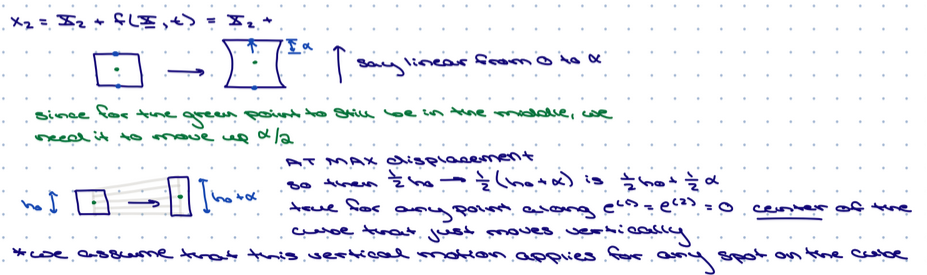
\includegraphics[scale=0.9]{Dawson-figures/1.png}

(An aside if that did not make sense in words: Expressed mathematically, if we consider the initial height of the HGC to be $h_0$, a point halfway up the initial cube is at $X_2 = \frac{1}{2}h_0$. The final height of the cube (at its maximum deformation) is then $h_0 + \alpha$, so for this point to remain halfway up the cube it is mapped to a final location of $x_2 = \frac{1}{2}(h_0 + \alpha) = \frac{1}{2}h_0 + \frac{1}{2}\alpha = X_2 + \frac{1}{2}\alpha$. So the point will move up by the same fraction of $\alpha$ that is its fraction of vertical height up the cube initially.)

This gives us the mapping function at maximum displacement of the cube, where we can note that the term $X_2 / h_0$ corresponds to the fraction "up that cube" that our initial material position is and that our initial height of the cube is $h_0 = 2$:
\begin{equation}
    x_2 = X_2 + \alpha \frac{X_2}{h_0} = X_2 + \alpha \frac{X_2}{2}
\end{equation}
Then putting in the sinusoidal dependence we get:
\begin{equation}
    x_2 = X_2 + \frac{\alpha X_2}{2} \sin{\omega t} = \chi_2(\bm{X},t)
\end{equation}

\emph{In the $\bm{e}^{(1)}$ and $\bm{e}^{(3)}$ directions}, we first note that the mapping functions should be the same. We also note that the displacement will be inwards, so a positive $X_1$ will have a negative change in position along $\bm{e}^{(1)}$ as it goes to $x_1$, and a negative $X_1$ will have a positive change in position along $\bm{e}^{(1)}$ as it goes to $x_1$. Once again, the mapping function will have the general form below, where $f(\bm{X},t)$ represents the change in position along $\bm{e}^{(1)}$:
\begin{equation}
    x_1 = X_1 + f(\bm{X},t)
\end{equation}

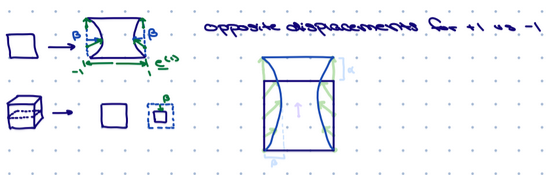
\includegraphics{Dawson-figures/2.png}

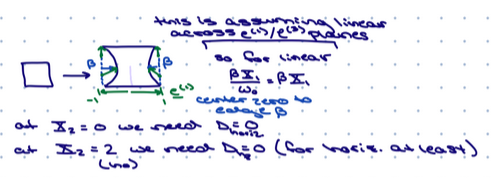
\includegraphics{Dawson-figures/3.png}

Along the center line ($X_1 = X_3 = 0$), $x_1 = X_1$ (ie. there is no lateral deformation). At the edge of the cube ($X_1 = X_3 = 1$) and halfway up the cube ($X_2 = 1$) there will be a maximum lateral deformation of $\beta$ ($x_1 = X_1 - \beta = 1-\beta$). We assume that all points in between are linearly related to these endpoints. That is, at $X_2 = 1$ we have a change in lateral position $-\beta X_1$. This gives us an equation for the maximum deformation thus far as:
\begin{equation}
    x_1 = X_1 - \beta X_1 X_2(t)
\end{equation}

The lateral displacement is also based on the vertical starting position, since at $X_2 = 0$ and $X_2 = 2$ we need $x_1 = X_1$ (no change in lateral position) with a maximum displacement in between these values. So, we also add in a parabolic function $X_2(t) = (X_2 - 2)(-x)$ to account for this dependence on vertical position. This gives us an expression for the maximum deformation:
\begin{equation}
    x_1 = X_1 + \beta X_1(X_2 - 2)(x)
\end{equation}
Where we can then add in the time-dependent sinusoidal dependence to get:
\begin{equation}
    x_1 = X_1 + \beta X_1(X_2 - 2)(x)\sin{\omega t} = \chi_1(\bm{X},t)
\end{equation}
Therefore, our overall mapping function $\bm{\chi}(\bm{X},t) = \bm{x}(t)$ is:
\begin{equation}
    \begin{split}
        x_1 = X_1 + \beta X_1(X_2 - 2)(x)\sin{\omega t} = \chi_1(\bm{X},t) \\
        x_2 = X_2 + \frac{\alpha}{2}X_2 \sin{\omega t} = \chi_2(\bm{X},t) \\
        x_3 = X_3 + \beta X_3(X_2 - 2)(x)\sin{\omega t} = \chi_3(\bm{X},t)
    \end{split}
\end{equation}

Then using this mapping function, we can calculate $\bn{F} = \gradX \space \bm{\chi}(\bm{X})$ by taking the corresponding partial derivatives of these components to get:

\begin{equation}
\bn{F} = 
\begin{bmatrix}
    1 + \beta X_2(X_2-2)\sin{\omega t} & \beta X_1 (2X_2-2)\sin{\omega t} & 0 \\
    0 & 1 + \frac{\alpha}{2}\sin{\omega t} & 0\\
    0 & \beta X_3 (2X_2-2)\sin{\omega t} & 1 + \beta X_2(X_2-2)\sin{\omega t}
\end{bmatrix}
\end{equation}
\hspace*{\fill} $\bigstar$

\medskip
(b) Determine the stretch magnitude of a small fiber positioned at a height $X_2 = 1$ and oriented at an angle $\theta$ from the $\bm{e}_1$ axis (in either the $\bm{e}_1- \bm{e}_2$ or $\bm{e}_1- \bm{e}_3$ plane). \newline
We first note that the stretch magnitude is $ \lambda (\bm{\hat{n}}) = \sqrt{\bm{\hat{n}} \cdot \bn{C} \bm{\hat{n}}}$ with $\bn{C} = \bn{F}^T\bn{F}$. Using our $\bn{F}$ from part (a), we note that $\bn{F}$ at $X_2 = 1$ is:
\begin{equation}
\bn{F} = 
\begin{bmatrix}
    1 - \beta \sin{\omega t} & 0 & 0 \\
    0 & 1 + \frac{\alpha}{2}\sin{\omega t} & 0\\
    0 & 0 & 1 - \beta \sin{\omega t}
\end{bmatrix}
\end{equation}
Which is also equal to $\bn{F}^T$ since it is a symmetric (and diagonal!) tensor. We can then calculate $\bn{C}$ as:
\begin{equation}
\bn{C} = \bn{F}^T\bn{F} = 
\begin{bmatrix}
    (1 - \beta \sin{\omega t})^2 & 0 & 0 \\
    0 & (1 + \frac{\alpha}{2}\sin{\omega t})^2 & 0\\
    0 & 0 & (1 - \beta \sin{\omega t})^2
\end{bmatrix}
\end{equation}
Then for $\bm{\hat{n}}$ in the $\bm{e}_1- \bm{e}_3$ plane we can note from the following sketch and some trigonometry that the unit vector should be:

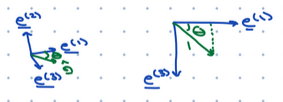
\includegraphics{Dawson-figures/BASIS.png}

\begin{equation}
    \bm{\hat{n}} = \cos{\theta}\bm{e}^{(1)} + 0\bm{e}^{(2)} + \sin{\theta}\bm{e}^{(3)}
\end{equation}
Then we can calculate $ \lambda (\bm{\hat{n}}) = \sqrt{\bm{\hat{n}} \cdot \bn{C} \bm{\hat{n}}}$ as follows:
\begin{equation}
    \bn{C}\bm{\hat{n}} = 
    \begin{bmatrix}
        \cos{\theta}(1 - \beta \sin{\omega t})^2 \\
        0 \\
         \sin{\theta}(1 - \beta \sin{\omega t})^2
    \end{bmatrix}
\end{equation}
\begin{equation}
    \bm{\hat{n}} \cdot \bn{C}\bm{\hat{n}} = 
        \cos^2{\theta}(1 - \beta \sin{\omega t})^2 + \sin^2{\theta}(1 - \beta \sin{\omega t})^2
\end{equation}
\begin{equation}
    \lambda (\bm{\hat{n}}) = \sqrt{\bm{\hat{n}} \cdot \bn{C} \bm{\hat{n}}} =  
        \sqrt{\cos^2{\theta}(1 - \beta \sin{\omega t})^2 + \sin^2{\theta}(1 - \beta \sin{\omega t})^2}
\end{equation}
Then we can simplify using the identity $\cos^2{\theta} + \sin^2{\theta} = 1$ to get:
\begin{equation}
    \lambda (\bm{\hat{n}}) = \sqrt{\bm{\hat{n}} \cdot \bn{C} \bm{\hat{n}}} =  
        \sqrt{ (\cos^2{\theta} + \sin^2{\theta})(1 - \beta \sin{\omega t})^2} = \sqrt{ (1 - \beta \sin{\omega t})^2} = (=1 - \beta \sin{\omega t}
\end{equation}
This is our $\lambda$ in the $\bm{e}_1- \bm{e}_3$ plane.
\hspace*{\fill} $\bigstar$

\medskip
(c) Determine the Lagrange-Green strain tensor $\bn{E}$ and the material logarithmic strain tensor $\bn{E}_H = \ln (\bn{U})$ for the geometric center $\bm{X}_c$ of the HGC. 
What are the maximum and minimum values of the strain eigenvalues $E_i(t)$ and $E_i^H(t)$? 
Would you expect one set to be more symmetric about zero as $\alpha$ gets large, and why? \newline
Note that the definition of the  Lagrange-Green strain tensor is $\bn{E} = \frac{1}{2}(\bn{C} - \bn{I})$. Using our $\bn{C}$ from part (b) we can calculate:
\begin{equation}
\bn{E} = (1/2) (
\begin{bmatrix}
    (1 - \beta \sin{\omega t})^2 & 0 & 0 \\
    0 & (1 + \frac{\alpha}{2}\sin{\omega t})^2 & 0\\
    0 & 0 & (1 - \beta \sin{\omega t})^2
\end{bmatrix} -
\begin{bmatrix}
    1 & 0 & 0 \\
    0 & 1 & 0\\
    0 & 0 & 1
\end{bmatrix} )
% \begin{bmatrix}
%     (1 - \beta \sin{\omega t})^2 -1 & 0 & 0 \\
%     0 & (1 + \frac{\alpha}{2}\sin{\omega t})^2 -1& 0\\
%     0 & 0 & (1 - \beta \sin{\omega t})^2 -1
% \end{bmatrix} )
\end{equation}

Performing this subtraction:
\begin{equation}
\bn{E} = (1/2)
\begin{bmatrix}
    (1 - \beta \sin{\omega t})^2 -1 & 0 & 0 \\
    0 & (1 + \frac{\alpha}{2}\sin{\omega t})^2 -1& 0\\
    0 & 0 & (1 - \beta \sin{\omega t})^2 -1
\end{bmatrix}
\end{equation}

Using that $a^2 - b^2 = (a+b)(a-b)$:
\begin{equation}
\bn{E} = (1/2)
\begin{bmatrix}
    (2 - \beta \sin{\omega t})(-\beta \sin{\omega t}) & 0 & 0 \\
    0 & (2 + \frac{\alpha}{2}\sin{\omega t})(\frac{\alpha}{2}\sin{\omega t})& 0\\
    0 & 0 & (2 - \beta \sin{\omega t})(-\beta \sin{\omega t})
\end{bmatrix}
\end{equation}
And applying the scalar multiplication by $1/2$ and simplifying:
\begin{equation}
\bn{E} =
\begin{bmatrix}
    (\beta \sin{\omega t}-2)(\frac{\beta}{2} \sin{\omega t}) & 0 & 0 \\
    0 & (2 + \frac{\alpha}{2}\sin{\omega t})(\frac{\alpha}{4}\sin{\omega t})& 0\\
    0 & 0 & (\beta \sin{\omega t}-2)(\frac{\beta}{2} \sin{\omega t})
\end{bmatrix}
\end{equation}
\hspace*{\fill} $\bigstar$

Note that the definition of the  material logarithmic strain tensor is $\bn{E}_H = \ln (\bn{U})$ with $\bn{U}$ the right stretch tensor. Since $\bn{C} = \bn{F}^T\bn{F} = \bn{U}^2$ and $\bn{F}$ is symmetric for the geometric center $\bn{X}_C$ (since there $X_2 = 1$, so it is the same simplified $\bn{F}$ as in part (b)) we can note that $\bn{C} = \bn{F}^2 = \bn{U}^2$ so $\bn{F} = \bn{U}$.
\begin{equation}
\bn{F} = \bn{U} =
\begin{bmatrix}
    1 - \beta \sin{\omega t} & 0 & 0 \\
    0 & 1 + \frac{\alpha}{2}\sin{\omega t} & 0\\
    0 & 0 & 1 - \beta \sin{\omega t}
\end{bmatrix}
\end{equation}
Then $\bn{E}_H = \ln (\bn{F})$ with $\bn{F}$ also a diagonal matrix, so we can just take the natural log of the diagonal components.
\begin{equation}
\bn{E}_H =\ln
\begin{bmatrix}
    1 - \beta \sin{\omega t} & 0 & 0 \\
    0 & 1 + \frac{\alpha}{2}\sin{\omega t} & 0\\
    0 & 0 & 1 - \beta \sin{\omega t}
\end{bmatrix} = 
\begin{bmatrix}
    \ln(1 - \beta \sin{\omega t}) & 0 & 0 \\
    0 & \ln(1 + \frac{\alpha}{2}\sin{\omega t}) & 0\\
    0 & 0 & \ln(1 - \beta \sin{\omega t})
\end{bmatrix}
\end{equation}
\hspace*{\fill} $\bigstar$

Then, for the minimum and maximum eigenvalues, we first note that these are both diagonal matrices and that the eigenvalues of a diagonal matrix will be the entries along the diagonal.

For $\bn{E}$, the eigenvalues are $\{(\beta \sin{\omega t}-2)(\frac{\beta}{2} \sin{\omega t}), (2 + \frac{\alpha}{2}\sin{\omega t})(\frac{\alpha}{4}\sin{\omega t}) \}$. To find the minimum and maximum eigenvalues, we check the extreme values of $\sin{\omega t}$, $\beta$, and $\alpha$. For the purposes of making this problem physically reasonable, assume that we can have $\beta$ values from $[0,1]$ and $\alpha$ values from $[0,2]$ (a maximum reasonable $\alpha$ of $2\beta$). $\sin{\omega t}$ will be on the domain $[-1,1]$.

For $\sin{\omega t} = 0$ we have eigenvalues $\{0, 0\}$.

For $\sin{\omega t} = 1$ we have eigenvalues $\{(\beta-2)(\beta/2), (2+\alpha/2)(\alpha/4)\}$. For $\beta = 0$ we get a first eigenvalue of $0$. For $\beta = 1$ we get a first eigenvalue of $-1/2$. For $\alpha = 0$ we get a second eigenvalue of $0$. For $\alpha = 2$ we get a second eigenvalue of $3/2$.

For $\sin{\omega t} = -1$ we have eigenvalues $\{(-\beta-2)(-\beta/2), (2-\alpha/2)(-\alpha/4)\}$ For $\beta = 0$ we get a first eigenvalue of $0$. For $\beta = 1$ we get a first eigenvalue of $3/2$. For $\alpha = 0$ we get a second eigenvalue of $0$. For $\alpha = 2$ we get a second eigenvalue of $-1/2$.

So our maximum eigenvalue for $\bn{E}$ is $3/2$ and our minimum is $-1/2$. As $\alpha$ gets large (say $\alpha \to \infty$) our maximum eigenvalue also goes to $\infty$ but our minimum remains as $-1/2$.
\hspace*{\fill} $\bigstar$

For $\bn{E}_H$, the eigenvalues are $\{\ln(1-\beta\sin{\omega t}), \ln(1+\frac{\alpha}{2}\sin{\omega t}) \}$. Repeating a similar process we get the following.

For $\beta = 0$ we have a first eigenvalue of $0$.

For $\beta = 1$ we have a first eigenvalue $\ln(1-\sin{\omega t})$. For $\sin{\omega t} = 0$ we have a first eigenvalue $\ln(1)=0$. For $\sin{\omega t} = 1$ we have a first eigenvalue $\ln(2)$. For $\sin{\omega t} = -1$ we have a first eigenvalue $\ln(0)=-\infty$.

For $\alpha = 0$ we have a first eigenvalue of $0$.

For $\alpha = 2$ we have a first eigenvalue $\ln(1+\sin{\omega t})$. For $\sin{\omega t} = 0$ we have a first eigenvalue $\ln(1)=0$. For $\sin{\omega t} = 1$ we have a first eigenvalue $\ln(2)$. For $\sin{\omega t} = -1$ we have a first eigenvalue $\ln(0)=-\infty$.

So our maximum eigenvalue for $\bn{E}_H$ is $\ln(2)$ and our minimum is $-\infty$. As $\alpha$ gets large (say $\alpha \to \infty$) our maximum eigenvalue goes to $\infty$ and our minimum remains $-\infty$. This also means that $\bn{E}_H$ has a more symmetric set of eigenvalues about zero as $\alpha$ gets large.
\hspace*{\fill} $\bigstar$

\medskip
(d) Determine both the material point acceleration $\bm{A}(\bm{X}_1)$ at a point $\frac{1}{2} \bm{e}_1 + 2\bm{e}_2 + \frac{1}{2} \bm{e}_3$.  
The material point acceleration is defined as:
\begin{equation}
    \bm{A}(\bm{X},t) = \frac{\partial^2 \bm{\chi}}{\partial t^2}
\end{equation}
With components $A_i = \frac{\partial^2 \bm{\chi}_i}{\partial t^2}$.
Taking our second derivatives of each component for the mapping function we get:
\begin{equation}
\begin{split}
    A_1 = \frac{\partial^2}{\partial t^2} (X_1 + \beta X_1(X_2 - 2)(x)\sin{\omega t}) = -\beta \omega^2 X_1X_2(X_2-2)(\sin{\omega t}) \\
    A_2 = \frac{\partial^2}{\partial t^2} (X_2 + \frac{\alpha}{2}X_2 \sin{\omega t}) = -(\alpha /2)X_2\omega^2(\sin{\omega t}) \\
    A_3 = \frac{\partial^2}{\partial t^2} (X_3 + \beta X_3(X_2 - 2)(x)\sin{\omega t}) = -\beta \omega^2 X_3X_2(X_2-2)(\sin{\omega t})
\end{split}
\end{equation}
Evaluating this at the material point $\bm{X} = \frac{1}{2} \bm{e}_1 + 2\bm{e}_2 + \frac{1}{2} \bm{e}_3$, so components $X_1 = 1/2$, $X_2 = 2$, and $X_3 = 1/2$, we get:
\begin{equation}
\begin{split}
    A_1 = 0 \\
    A_2 = -\alpha \omega^2\sin{\omega t} \\
    A_3 = 0
\end{split}
\end{equation}
Giving us a material point acceleration vector of:
\begin{equation}
    \bm{A} = 0 \bm{e}_1 -\alpha \omega^2\sin{\omega t}\bm{e}_2 + 0\bm{e}_3
\end{equation}
\hspace*{\fill} $\bigstar$

% \end{document}

\end{document}

% Section 1 Notes
% by which the VE properties of MTs are established microtubules vary in exhibiting these properties

%These results indicate that individual microtubules might also exhibit viscoelastic behaviors.
%as well as a decreased persistence length
%individual \C{deacetylated} microtubules showed an increase in deformation 

% importnat for understanding networks and deformations over time? where would a MT act more independently rather than in a bundle though, or why would the single molecule mechanical properties actually matter?
% However, recent papers have demonstrated that individual microtubules might exhibit viscoelastic behaviors

% Microtuuuuuuuubles.
% Looking at them from a viscoelastic perspective, particularly in terms of relaxation.
% Single microtubules, but could also do networks or bundles that have already been looked at as viscoelastic?

\section{Introductory context}
\begin{itemize}
    \item Microtubules are intracellular filaments composed of tubulin subunits [\cite{rev_nogales}]. As the most rigid cytoskeletal filament [\cite{rev_mechanics}], microtubules serve multiple mechanical roles in cells including maintenance of cell shape [\cite{rev_org-shape}], generation of intracellular forces [\cite{rev_push-pull}], and cell migration [\cite{rev_migration}]. Despite their relative rigidity, microtubules can bend under intracellular forces [\cite{p_bend-in-cells}]. This bending is functionally important in platelets [\cite{rev_platelet-MTs}] and cardiomyocytes [\cite{rev_carmy-MTs}].
    \item Measurements of microtubule mechanical properties have focused on their flexural rigidity [\cite{p_thermal-flex}], and experimental papers generally model microtubules as thin elastic beams [\cite{rev_mechanics}]. However, measurements of microtubule mechanics over the past couple of decades are and have remained highly variable [\cite{rev_hawkins}]. More recent work has tried to address these discrepancies by investigating different factors that could impact mechanics, including polymerization rate [\cite{p_growth-rate-1, p_growth-rate-2}], temperature [\cite{p_temp}], salt concentration [\cite{p_salt}], presence of stabilizing agents [\cite{p_stabilize}], and microtubule length [\cite{p_length-1}]. Other papers have noted behaviors that contradict with the view of microtubules as purely elastic materials, including strain-dependent responses [\cite{p_strain-soften}] and increased deformation with repeated bending [\cite{p_repeated-flow}].
\end{itemize}

\section{The state of the field}
\begin{itemize}
    \item The most common experimental methods to measure microtubule mechanics are thermal fluctuations [\cite{p_thermal-flex, p_therm-flex-2}], hydrodynamic flow [\cite{p_flow-1}], and optical trapping [\cite{p_trap-1, p_trap-2}].
    \item Although microtubules are often treated as elastic beams in experimental papers [\cite{rev_mechanics}], other models of microtubule behaviors have been published. Current models of microtubule bending include (1) molecular dynamics or other atomic models [\cite{p_Molec-Dyn-1, p_atomic-1}], (2) models noting the interactions of the thinner protofilaments composing microtubules [\cite{p_protofil-1, p_protofil-2}], and (3) continuum models focusing on the anisotropic elastic properties of microtubules [\cite{p_aniso-2, p_aniso-3, p_aniso-4}]. Viscoelastic models of microtubules have generally been restricted to microtubule networks [\cite{rev_visco, p_visco-network}], models considering the viscous properties of the surrounding cytosol [\cite{p_visco-cytosol}], or models looking at cell-type specific configurations of microtubule bundles [\cite{p_visco-bundle, p_visco-myocyte}]. At least one paper proposed a viscoelastic model for microtubule bending, although without specific paired experiments [\cite{p_visco-model}].
\end{itemize}

\section{The Big Gap}
\begin{itemize}
    \item As far as I am aware, it remains to be directly experimentally tested whether single microtubules demonstrate elastic or viscoelastic behaviors.
    \item The most challenging barrier to doing these experiments seems to be the availability of techniques for making such measurements.
    \item As a note, I'm slightly less sure that my proposed project will be novel given what I found in the literature so far. It seems quite possible that, with a little more looking, I could find that it has already been done. Any suggestions on how to push the project a little farther to address this would be greatly appreciated!
    % \item I should note, the more papers I find the more I am wondering if this *has* been addressed already. 
\end{itemize}

% While a few viscoelastic models have been proposed and aspects of multiple experiments suggest the potential for microtubules to be viscoelastic, 

\begin{thebibliography}{00} % using Chicago 18th shortened from Zotero

\bibitem[Nogales, 2025]{rev_nogales}
Nogales, Eva. Structural Insights into Microtubule Function. 2025. % review, general microtubules. Roles in cell shape, transport, motility, division.

\bibitem[Romet-Lemonne et al., 2025]{rev_mechanics}
Romet-Lemonne, Guillaume, Cécile Leduc, Antoine Jégou, and Hugo Wioland. “Mechanics of Single Cytoskeletal Filaments.” Annual Review of Biophysics 54, no. 1 (2025): 303–27. https://doi.org/10.1146/annurev-biophys-030722-120914. % review, mechanics of microtubules (focus on mechanical properties rather than functional roles of microtubule mechanics)

\bibitem[Akhmanova and Kapitein, 2022]{rev_org-shape}
Akhmanova, Anna, and Lukas C. Kapitein. “Mechanisms of Microtubule Organization in Differentiated Animal Cells.” Nature Reviews Molecular Cell Biology 23, no. 8 (2022): 541–58. https://doi.org/10.1038/s41580-022-00473-y.

\bibitem[Gudimchuk et al., 2023]{rev_push-pull}
Gudimchuk, Nikita B., and Veronika V. Alexandrova. “Measuring and Modeling Forces Generated by Microtubules.” Biophysical Reviews 15, no. 5 (2023): 1095–110. https://doi.org/10.1007/s12551-023-01161-7. % review, force generation by microtubules

\bibitem[Schmidt and Stehbens, 2024]{rev_migration}
Schmidt, Christanny J., and Samantha J. Stehbens. “Microtubule Control of Migration: Coordination in Confinement.” Current Opinion in Cell Biology 86 (February 2024): 102289. https://doi.org/10.1016/j.ceb.2023.102289. % review

\bibitem[Pallavicini et al., 2014]{p_bend-in-cells}
Pallavicini, Carla, Valeria Levi, Diana E. Wetzler, et al. “Lateral Motion and Bending of Microtubules Studied with a New Single-Filament Tracking Routine in Living Cells.” Biophysical Journal 106, no. 12 (2014): 2625–35. https://doi.org/10.1016/j.bpj.2014.04.046. % primary

\bibitem[Sadoul, 2015]{rev_platelet-MTs}
Sadoul, K. “New Explanations for Old Observations: Marginal Band Coiling during Platelet Activation.” Journal of Thrombosis and Haemostasis 13, no. 3 (2015): 333–46. https://doi.org/10.1111/jth.12819. % review, microtubules in platelet shape

\bibitem[Uchida et al., 2022]{rev_carmy-MTs}
Uchida, Keita, Emily A. Scarborough, and Benjamin L. Prosser. “Cardiomyocyte Microtubules: Control of Mechanics, Transport, and Remodeling.” Annual Review of Physiology 84, no. Volume 84, 2022 (2022): 257–83. https://doi.org/10.1146/annurev-physiol-062421-040656. % review, microtubules in cardiomyocyte contractility

\bibitem[Gittes et al., 1993]{p_thermal-flex}
Gittes, F, B Mickey, J Nettleton, and J Howard. “Flexural Rigidity of Microtubules and Actin Filaments Measured from Thermal Fluctuations in Shape.” Journal of Cell Biology 120, no. 4 (1993): 923–34. https://doi.org/10.1083/jcb.120.4.923.

\bibitem[Hawkins et al., 2010]{rev_hawkins}
Hawkins, Taviare, Matthew Mirigian, M. Selcuk Yasar, and Jennifer L. Ross. “Mechanics of Microtubules.” Journal of Biomechanics 43, no. 1 (2010): 23–30. https://doi.org/10.1016/j.jbiomech.2009.09.005. % review, differences in measurements of mechanical properties

\bibitem[Zhou et al., 2021]{p_growth-rate-1}
Zhou, Hang, Naoto Isozaki, Kazuya Fujimoto, and Ryuji Yokokawa. “Growth Rate-Dependent Flexural Rigidity of Microtubules Influences Pattern Formation in Collective Motion.” Journal of Nanobiotechnology 19, no. 1 (2021): 218. https://doi.org/10.1186/s12951-021-00960-y.

\bibitem[Janson and Dogterom, 2004]{p_growth-rate-2}
Janson, Marcel E., and Marileen Dogterom. “A Bending Mode Analysis for Growing Microtubules: Evidence for a Velocity-Dependent Rigidity.” Biophysical Journal 87, no. 4 (2004): 2723–36. https://doi.org/10.1529/biophysj.103.038877.

\bibitem[Kawaguchi et al., 2008]{p_temp}
Kawaguchi, Kenji, Shin’ichi Ishiwata, and Toshihide Yamashita. “Temperature Dependence of the Flexural Rigidity of Single Microtubules.” Biochemical and Biophysical Research Communications 366, no. 3 (2008): 637–42. https://doi.org/10.1016/j.bbrc.2007.11.162.

\bibitem[Harris et al., 2018]{p_salt}
Harris, Brandon J., Jennifer L. Ross, and Taviare L. Hawkins. “Microtubule Seams Are Not Mechanically Weak Defects.” Physical Review E 97, no. 6 (2018): 062408. https://doi.org/10.1103/PhysRevE.97.062408.

\bibitem[Mickey and Howard, 1995]{p_stabilize}
Mickey, B., and J. Howard. “Rigidity of Microtubules Is Increased by Stabilizing Agents.” The Journal of Cell Biology 130, no. 4 (1995): 909–17. https://doi.org/10.1083/jcb.130.4.909.

\bibitem[Pampaloni et al., 2006]{p_length-1}
Pampaloni, Francesco, Gianluca Lattanzi, Alexandr Jonáš, Thomas Surrey, Erwin Frey, and Ernst-Ludwig Florin. “Thermal Fluctuations of Grafted Microtubules Provide Evidence of a Length-Dependent Persistence Length.” Proceedings of the National Academy of Sciences 103, no. 27 (2006): 10248–53. https://doi.org/10.1073/pnas.0603931103. % primary, length dependent persistence length

\bibitem[Memet et al., 2018]{p_strain-soften}
Memet, Edvin, Feodor Hilitski, Margaret A Morris, Walter J Schwenger, Zvonimir Dogic, and L Mahadevan. “Microtubules Soften Due to Cross-Sectional Flattening.” eLife 7 (June 2018): e34695. https://doi.org/10.7554/eLife.34695. % softening at high strains? is the critical strain biologically relavent?

\bibitem[Portran et al., 2017]{p_repeated-flow}
Portran, Didier, Laura Schaedel, Zhenjie Xu, Manuel Théry, and Maxence V. Nachury. “Tubulin Acetylation Protects Long-Lived Microtubules against Mechanical Ageing.” Nature Cell Biology 19, no. 4 (2017): 391–98. https://doi.org/10.1038/ncb3481. % primary, acetylation as a tubulin PTM impacts mechanical properties AND change in bending with repeated flow cycles

\bibitem[Valdman et al., 2012]{p_therm-flex-2}
Valdman, David, Paul J. Atzberger, Dezhi Yu, Steve Kuei, and Megan T. Valentine. “Spectral Analysis Methods for the Robust Measurement of the Flexural Rigidity of Biopolymers.” Biophysical Journal 102, no. 5 (2012): 1144–53. https://doi.org/10.1016/j.bpj.2012.01.045.

\bibitem[Venier et al., 1994]{p_flow-1}
Venier, P., A.C. Maggs, M.F. Carlier, and D. Pantaloni. “Analysis of Microtubule Rigidity Using Hydrodynamic Flow and Thermal Fluctuations.” Journal of Biological Chemistry 269, no. 18 (1994): 13353–60. https://doi.org/10.1016/S0021-9258(17)36840-0.

\bibitem[Kurachi et al., 1995]{p_trap-1}
Kurachi, Masashi, Masayuki Hoshi, and Hideo Tashiro. “Buckling of a Single Microtubule by Optical Trapping Forces: Direct Measurement of Microtubule Rigidity.” Cell Motility 30, no. 3 (1995): 221–28. https://doi.org/10.1002/cm.970300306.

\bibitem[van Mameren et al., 2009]{p_trap-2}
van Mameren, Joost van, Karen C. Vermeulen, Fred Gittes, and Christoph F. Schmidt. “Leveraging Single Protein Polymers To Measure Flexural Rigidity.” The Journal of Physical Chemistry B 113, no. 12 (2009): 3837–44. https://doi.org/10.1021/jp808328a.

\bibitem[Septh and MacKintosh, 2010]{p_Molec-Dyn-1}
Sept, David, and Fred C. MacKintosh. “Microtubule Elasticity: Connecting All-Atom Simulations with Continuum Mechanics.” Physical Review Letters 104, no. 1 (2010): 018101. https://doi.org/10.1103/PhysRevLett.104.018101.

\bibitem[Molodtsov et al., 2005]{p_atomic-1}
Molodtsov, Maxim I., Elena A. Ermakova, Emmanuil E. Shnol, Ekaterina L. Grishchuk, J. Richard McIntosh, and Fazly I. Ataullakhanov. “A Molecular-Mechanical Model of the Microtubule.” Biophysical Journal 88, no. 5 (2005): 3167–79. https://doi.org/10.1529/biophysj.104.051789.

% \bibitem[Li et al., 2006]{p_aniso-1}
% Li, C., C.Q. Ru, and A. Mioduchowski. “Length-Dependence of Flexural Rigidity as a Result of Anisotropic Elastic Properties of Microtubules.” Biochemical and Biophysical Research Communications 349, no. 3 (2006): 1145–50. https://doi.org/10.1016/j.bbrc.2006.08.153. % primary, reported difference sin flexural rigidity due to inaccuracy of isotropic beam model for shorter microtubule lengths, and that longitudinal (rather than circumferential) Young's modulus is length-independent due to anisotropic elastic properties of microtubules

\bibitem[Wang et al., 2006]{p_aniso-2}
Wang, C.Y., C.Q. Ru, and A. Mioduchowski. “Orthotropic Elastic Shell Model for Buckling of Microtubules.” Physical Review E 74, no. 5 (2006): 052901. https://doi.org/10.1103/PhysRevE.74.052901. % primary, anisotropic elastic shell model rather than isotropic elastic shell model (similar to other paper)

\bibitem[Liew et al., 2011]{p_aniso-3}
Liew, K.M., Ping Xiang, and Yuzhou Sun. “A Continuum Mechanics Framework and a Constitutive Model for Predicting the Orthotropic Elastic Properties of Microtubules.” Composite Structures 93, no. 7 (2011): 1809–18. https://doi.org/10.1016/j.compstruct.2011.01.017. % primary

\bibitem[Deriu et al., 2010]{p_aniso-4}
Deriu, Marco A., Monica Soncini, Mario Orsi, et al. “Anisotropic Elastic Network Modeling of Entire Microtubules.” Biophysical Journal 99, no. 7 (2010): 2190–99. https://doi.org/10.1016/j.bpj.2010.06.070.

\bibitem[Wang et al., 2016]{p_protofil-1}
Wang, Chengyuan, Zhigang Guo, Ruijie Wang, and Ying Luo. “Role of the Inter-Protofilament Sliding in the Bending of Protein Microtubules.” Journal of Biomechanics 49, no. 16 (2016): 3803–7. https://doi.org/10.1016/j.jbiomech.2016.10.008.

\bibitem[Ye et al., 2025]{p_protofil-2}
Ye, Yucheng, Zheng Hao, Jingyi Luo, et al. “Tubulin Isotypes of C. Elegans Harness the Mechanosensitivity of the Lattice for Microtubule Luminal Accessibility.” Nature Physics, ahead of print, August 26, 2025. https://doi.org/10.1038/s41567-025-02983-w.

\bibitem[Liew et al., 2015]{rev_models}
Liew, K.M., Ping Xiang, and L.W. Zhang. “Mechanical Properties and Characteristics of Microtubules: A Review.” Composite Structures 123 (May 2015): 98–108. https://doi.org/10.1016/j.compstruct.2014.12.020. % review

\bibitem[Corominas-Murtra and Petridou, 2021]{rev_visco}
Corominas-Murtra, Bernat, and Nicoletta I. Petridou. “Viscoelastic Networks: Forming Cells and Tissues.” Frontiers in Physics 9 (2021). https://doi.org/10.3389/fphy.2021.666916. % review, actin and vimentin at single filament level show nonlinear increase in shear modulus at different strain amplitudes, an dmore appaent at network level with crosslinks influencing viscoelastic behavior of network. Transient and non-covalent crosslinking interactions to form viscoelastic material whereas covalent an elastic material. **NOT READ**

\bibitem[Lin et al., 2007]{p_visco-network}
Lin, Yi-Chia, Gijsje H. Koenderink, Frederick C. MacKintosh, and David A. Weitz. “Viscoelastic Properties of Microtubule Networks.” Macromolecules 40, no. 21 (2007): 7714–20. https://doi.org/10.1021/ma070862l. % primary, linear viscoelastic properties of microtubule networks

\bibitem[Li, 2008]{p_visco-cytosol}
Li, Teng. “A Mechanics Model of Microtubule Buckling in Living Cells.” Journal of Biomechanics 41, no. 8 (2008): 1722–29. https://doi.org/10.1016/j.jbiomech.2008.03.003.

\bibitem[Shamloo et al., 2015]{p_visco-bundle}
Shamloo, Amir, Farid Manuchehrfar, and Hashem Rafii-Tabar. “A Viscoelastic Model for Axonal Microtubule Rupture.” Journal of Biomechanics 48, no. 7 (2015): 1241–47. https://doi.org/10.1016/j.jbiomech.2015.03.007.

\bibitem[Caporizzo et al., 2018]{p_visco-myocyte}
Caporizzo, Matthew Alexander, Christina Yingxian Chen, Alexander Koizumi Salomon, Kenneth B. Margulies, and Benjamin L. Prosser. “Microtubules Provide a Viscoelastic Resistance to Myocyte Motion.” Biophysical Journal 115, no. 9 (2018): 1796–807. https://doi.org/10.1016/j.bpj.2018.09.019.

\bibitem[Abdelmalek et al., 2021]{p_visco-model}
Abdelmalek, Zahra, Mohammed Karbon, Arameh Eyvazian, Ali Forooghi, Hamed Safarpour, and Iskander Tlili. “On the Dynamics of a Curved Microtubule-Associated Proteins by Considering Viscoelastic Properties of the Living Biological Cells.” Journal of Biomolecular Structure and Dynamics 39, no. 7 (2021): 2415–29. https://doi.org/10.1080/07391102.2020.1747549.


\bibliographystyle{elsarticle-harv} 
% \bibliography{cas-refs}
\end{thebibliography}

% \end{document}


% do they compress with bending?
% Functional roles are based on proteins and motors bound to microtubules [ ] as well as the in
    
    % include transport in cells [\cite{rev_transport}], cell migration [/cite{rev_migration}], maintenance of cell shape, cell division, and more. While some of these roles result from other proteins or motors bound to microtubules.

%     Microtubules are dynamic intracellular filaments composed of tubulin subunits [\cite{rev_nogales}]. As the most rigid cytoskeleton filament [], a primary cellular role is as pathways for intracellular transport []. However, microtubules also have multiple mechanical roles in cells, including maintenance of cell shape [multiple], generation of pushing and pulling forces [], and providing compressive resistance to bending []. Despite their relative rigidity, microtubules are also bendable under intracellular forces [bending in cells]. This ability to bend serves functional roles in platelets [] and cardiomyocytes [].  %Microtubules in cells perform functional roles as cross-linked networks [], filamentous bundles [], and other configurations [].

% %    
    
%     \item While some mechanical functions are based on cross-linked networks of microtubules [], many microtubules work individually or in small groups [Hawkins plus others, do find those citations though]. The lack of need to cross link based in stiffness according to Gittes [Gittes for history]. Microtubules also not extendable and filaments either bend or slide between each other rather than induvidually stretch [also gittes]. More recent measurements acknowledge something beyond elastic beams. Emerging work trying to address to discrepencies in measurements by looking at different factors could depend on. [Zhou, growth rate]

    %    The mechanical properties of single microtubules are most commonly measured through optical trapping [], hydrodynamic flow [], or thermal fluctuations []. Current measurements of bending modulus are highly variable []. Experimental papers will commonly characterize microtubule bending as that of an isotropic elastic rod [multiple]. This inconsistency, along with studies noting the potential for anisotropic behaviors [] and smaller-scale mechanical interactions [], suggest a requirement for more comprehensive physical models of their mechanical behavior. [Memet cross sectional flattening, deviate from simple elastic model with softening response captured by flattening, ALSO strain magnitude dependence] [so some folks have already looked...wasn't there one for cardiomyocytes that had a VE regime, was that for single or bundles]




% %%%% Additions
% \bibitem[Ye et al., 2025]{p_lumen}
% Ye, Yucheng, Zheng Hao, Jingyi Luo, et al. “Tubulin Isotypes of C. Elegans Harness the Mechanosensitivity of the Lattice for Microtubule Luminal Accessibility.” Nature Physics, ahead of print (2025). https://doi.org/10.1038/s41567-025-02983-w. % primary, tubulin isotypes and mechanics as well as protofilament interactions during bending for different isotypes
% Nishida, Kohei, Kosuke Matsumura, Miki Tamura, et al. “Effects of Three Microtubule-Associated Proteins (MAP2, MAP4, and Tau) on Microtubules’ Physical Properties and Neurite Morphology.” Scientific Reports 13, no. 1 (2023): 8870. https://doi.org/10.1038/s41598-023-36073-9.
% \bibitem[]{}
% Xu, Zhenjie, Laura Schaedel, Didier Portran, et al. “Microtubules Acquire Resistance from Mechanical Breakage through Intralumenal Acetylation.” Science 356, no. 6335 (2017): 328–32. https://doi.org/10.1126/science.aai8764. % primary, acetylation as a tubulin PTM impacts mechanical properties
% \bibitem[]{}
% Xu, Zhenjie, Laura Schaedel, Didier Portran, et al. “Microtubules Acquire Resistance from Mechanical Breakage through Intralumenal Acetylation.” Science 356, no. 6335 (2017): 328–32. https://doi.org/10.1126/science.aai8764.
% \bibitem[]{}
% Mehrbod, Mehrdad, and Mohammad R. K. Mofrad. “On the Significance of Microtubule Flexural Behavior in Cytoskeletal Mechanics.” PLOS ONE 6, no. 10 (2011): e25627. https://doi.org/10.1371/journal.pone.0025627. % buckling modes?

% %%% Microtubules in general
% \bibitem[Agrawal et al., 2022]{rev_transport}
% Agrawal, Anamika, Zubenelgenubi C. Scott, and Elena F. Koslover. “Morphology and Transport in Eukaryotic Cells.” Annual Review of Biophysics 51, no. Volume 51, 2022 (2022): 247–66. https://doi.org/10.1146/annurev-biophys-111121-103956. % review, transport in cells
% \bibitem[]{}
% Sulerud, Taylor, Abdullah Bashar Sami, Guihe Li, April Kloxin, John Oakey, and Jesse Gatlin. “Microtubule-Dependent Pushing Forces Contribute to Long-Distance Aster Movement and Centration in Xenopus Laevis Egg Extracts.” Molecular Biology of the Cell 31, no. 25 (2020): 2791–802. https://doi.org/10.1091/mbc.E20-01-0088. % primary, cell division centering based on microtubule based pushing mechanisms
% \bibitem[]{}
% Rodionov, V I, F K Gyoeva, E Tanaka, A D Bershadsky, J M Vasiliev, and V I Gelfand. “Microtubule-Dependent Control of Cell Shape and Pseudopodial Activity Is Inhibited by the Antibody to Kinesin Motor Domain.” The Journal of Cell Biology 123, no. 6 (1993): 1811–20. https://doi.org/10.1083/jcb.123.6.1811. % primary, cell shape also requires motors
% \bibitem[Behnke]{p_platelet-MB}
% Behnke, O. “A Comparative Study of Microtubules of Disk-Shaped Blood Cells.” Journal of Ultrastructure Research 31, nos. 1–2 (1970): 61–75. https://doi.org/10.1016/S0022-5320(70)90145-0. % primary, marginal band required for cell shape in SOME cell types, including platelets
% \bibitem[]{p_platelet-shape}
% Italiano, Joseph E., Jr, Wolfgang Bergmeier, Sanjay Tiwari, et al. “Mechanisms and Implications of Platelet Discoid Shape.” Blood 101, no. 12 (2003): 4789–96. https://doi.org/10.1182/blood-2002-11-3491. % primary

% %%% Tubulin Code
% \bibitem[]{}
% Janke, Carsten, and Maria M. Magiera. “The Tubulin Code and Its Role in Controlling Microtubule Properties and Functions.” Nature Reviews Molecular Cell Biology 21, no. 6 (2020): 307–26. https://doi.org/10.1038/s41580-020-0214-3. % review, overall tubulin code
% \bibitem[]{}
% Gasic, Ivana. “Regulation of Tubulin Gene Expression: From Isotype Identity to Functional Specialization.” Frontiers in Cell and Developmental Biology 10 (May 2022). https://doi.org/10.3389/fcell.2022.898076. % review, functional specialization from different isotypes **NOT READ**
% \bibitem[]{}
% Janke, Carsten, and Jeannette Chloë Bulinski. “Post-Translational Regulation of the Microtubule Cytoskeleton: Mechanisms and Functions.” Nature Reviews Molecular Cell Biology 12, no. 12 (2011): 773–86. https://doi.org/10.1038/nrm3227. % review, functional specialization from different PTMS **NOT READ**

% %%% Mechanical Properties

% %%% Mechanical Roles
% \bibitem[]{}
% Matis, Maja. “The Mechanical Role of Microtubules in Tissue Remodeling.” BioEssays 42, no. 5 (2020): 1900244. https://doi.org/10.1002/bies.201900244. % review, microtubules in cellular trafficking and signaling during tissue formation as well as direct mechanical roles **NOT READ**

% \bibitem[]{}
% Garcin, Clare, and Anne Straube. “Microtubules in Cell Migration.” Essays in Biochemistry 63, no. 5 (2019): 509–20. https://doi.org/10.1042/EBC20190016. % review, microtubule roles in directed cell migration (as tracks for intracellular transport, force generation, compressive elements to support protrusions, and signaling) **NOT READ**

% %%% Health examples
% \bibitem[Caporizzo and Prosser, 2022]{card_HF}
% Caporizzo, Matthew A., and Benjamin L. Prosser. “The Microtubule Cytoskeleton in Cardiac Mechanics and Heart Failure.” Nature Reviews Cardiology 19, no. 6 (2022): 364–78. https://doi.org/10.1038/s41569-022-00692-y. % review, mechanical modulation of microtubules proposed as potential therapeutic target in heart failure

% %%% Microtubule networks

% %%% Tubulin structures
% \bibitem[]{}
% Alushin, Gregory M., Gabriel C. Lander, Elizabeth H. Kellogg, Rui Zhang, David Baker, and Eva Nogales. “High-Resolution Microtubule Structures Reveal the Structural Transitions in Αβ-Tubulin upon GTP Hydrolysis.” Cell 157, no. 5 (2014): 1117–29. https://doi.org/10.1016/j.cell.2014.03.053. % primary, structure and conformational changes with taxol binding and GTP hydrolysis

% %%% Existing measurements
% \bibitem[]{}
% Mameren, Joost van, Karen C. Vermeulen, Fred Gittes, and Christoph F. Schmidt. “Leveraging Single Protein Polymers To Measure Flexural Rigidity.” The Journal of Physical Chemistry B 113, no. 12 (2009): 3837–44. https://doi.org/10.1021/jp808328a. % primary, optical trapping

% %%% Existing models

% %%% Microtubule bundles
% \bibitem[]{}
% Soheilypour, Mohammad, Mohaddeseh Peyro, Stephen J. Peter, and Mohammad R.K. Mofrad. “Buckling Behavior of Individual and Bundled Microtubules.” Biophysical Journal 108, no. 7 (2015): 1718–26. https://doi.org/10.1016/j.bpj.2015.01.030. % primary

% %%% Microtubules in cells
% \bibitem[]{}
% Brangwynne, Clifford P., Frederick C. MacKintosh, Sanjay Kumar, et al. “Microtubules Can Bear Enhanced Compressive Loads in Living Cells Because of Lateral Reinforcement.” Journal of Cell Biology 173, no. 5 (2006): 733–41. https://doi.org/10.1083/jcb.200601060. % primary
% \bibitem[]{}
% Li, Teng. “A Mechanics Model of Microtubule Buckling in Living Cells.” Journal of Biomechanics 41, no. 8 (2008): 1722–29. https://doi.org/10.1016/j.jbiomech.2008.03.003. % primary

% %%% Other
% \bibitem[Okenve-Ramos et al, 2024]{neur_aging}
% Okenve-Ramos, Pilar, Rory Gosling, Monika Chojnowska-Monga, et al. “Neuronal Ageing Is Promoted by the Decay of the Microtubule Cytoskeleton.” PLOS Biology 22, no. 3 (2024): e3002504. https://doi.org/10.1371/journal.pbio.3002504. 
% \bibitem[]{}
% Needleman, Daniel J., Miguel A. Ojeda-Lopez, Uri Raviv, et al. “Synchrotron X-Ray Diffraction Study of Microtubules Buckling and Bundling under Osmotic Stress: A Probe of Interprotofilament Interactions.” Physical Review Letters 93, no. 19 (2004): 198104. https://doi.org/10.1103/PhysRevLett.93.198104. % primary, shape change with osmotic stress and looking at interprotofilament bond strengths
% \bibitem[]{}
% Mickey, B., and J. Howard. “Rigidity of Microtubules Is Increased by Stabilizing Agents.” The Journal of Cell Biology 130, no. 4 (1995): 909–17. https://doi.org/10.1083/jcb.130.4.909.

% % 
%     \item Some experiments have noted bending behaviors that would deviate from elastic behavior, including length-dependent elastic modulus [] and increased deformation with repeated bending []. There are currently multiple possible explanations for these deviations from elastic behavior, including isotropic assumptions in modeling [] or microtubule damage []. (also bending past thin beam model?)

%     %    
%     While the viscoelastic characteristics of cross-linked microtubule networks are established [multiple], similar investigations have not been performed for single microtubules.
%     \item The most challenging barrier in making such measurements is...? The high stiffness of microtubules makes these measurements more challenging than for other cytoskeletal filaments [], where time-dependent mechanical properties have also been established []. Is this true, check on that. Perhaps see if need to be characterized by more than a single number? What is the challenge then? Because some papers HAVE done stuff like that perhaps. But at least address the other changes? Memet and low/high strain regimes differences and their measurements, they have a model as well...so take another look at how what you're proposing actually addresses a gap or not, and if it doesn't, see what further steps you can take that would be VE/SM relevant! Go through that paper and see what some next steps might be. READ THROUGH MEMET AND CHECK THAT THEN ALSO SEE WHAT COULD GO A BIT FURTHER!!

\section*{Examples II: Kinetics, Constitutive Laws, and Viscoelasticity I}
\label{PS2}

\medskip
\subsection*{2--1. \textbf{Balance of mass}}
Local balance (or conservation) of mass states that
\begin{equation}
    \frac{\partial \rho}{\partial t} + \nabla_{\bm{x}} \cdot (\rho \bm{v}) = 0
\end{equation}
Using the product rule we can expand out the second term on the left hand side we get
\begin{equation}
    \frac{\partial \rho}{\partial t} + [\nabla_{\bm{x}} \rho \cdot \bm{v} + \rho (\nabla_{\bm{x}} \cdot \bm{v})] = 0
\end{equation}
Then apply the divergence in spherical coordinates, defined in Bower as $\nabla f = \bm{e_R}\frac{\partial f}{\partial R} + \bm{e_{\theta}}\frac{1}{R}\frac{\partial f}{\partial \theta} + \bm{e_{\phi}}\frac{1}{R\sin{\theta}}\frac{\partial f}{\partial \phi}$ for scalar functions and $\nabla \cdot \bm{v} \equiv \frac{\partial v_R}{\partial R} + 2\frac{v_R}{R} + \frac{1}{R}\frac{\partial v_{\theta}}{\partial \theta} + \frac{1}{R \sin{\theta}}\frac{\partial v_{\phi}}{\partial \phi} + \cot{\theta}\frac{v_{\theta}}{R}$ for vector functions, to get
\begin{equation}
    \frac{\partial \rho}{\partial t} + (\bm{e_r}\frac{\partial \rho}{\partial r} + \bm{e_{\theta}}\frac{1}{r}\frac{\partial \rho}{\partial \theta} + \bm{e_{\phi}}\frac{1}{r\sin{\theta}}\frac{\partial \rho}{\partial \phi})\cdot \bm{v} + \rho(\frac{\partial v_r}{\partial r} + 2\frac{v_r}{r} + \frac{1}{r}\frac{\partial v_{\theta}}{\partial \theta} + \frac{1}{r \sin{\theta}}\frac{\partial v_{\phi}}{\partial \phi} + \cot{\theta}\frac{v_{\theta}}{r})= 0
\end{equation}
Note that $\bm{v} = v_r \bm{e_r}$ in index notation and take the dot product
\begin{equation}
    \frac{\partial \rho}{\partial t} + (\frac{\partial \rho}{\partial r}v_r) + \rho(\frac{\partial v_r}{\partial r} + 2\frac{v_r}{r} + \frac{1}{r}\frac{\partial v_{\theta}}{\partial \theta} + \frac{1}{r \sin{\theta}}\frac{\partial v_{\phi}}{\partial \phi} + \cot{\theta}\frac{v_{\theta}}{r})= 0
\end{equation}
Then since our system is spherically symmetric, our velocity $\bm{v}$ will not change in the $\theta$ or $\phi$ directions. This means that $ \frac{\partial v_{\theta}}{\partial \theta}= \frac{\partial v_{\phi}}{\partial \phi} = 0$. In addition, the expansion velocity is only in the $\bm{e_r}$ direction, as defined in the problem by $\bm{v}(r,t) = v_r \bm{e_r}$, so $v_{\theta} = v_{\phi} =0$ as well.
\begin{equation}
    \frac{\partial \rho}{\partial t} + (\frac{\partial \rho}{\partial r}v_r) + \rho(\frac{\partial v_r}{\partial r} + 2\frac{v_r}{r})= 0
\end{equation}
Where we can pull out a $1/r$ from the third term to get
\begin{equation}
    \frac{\partial \rho}{\partial t} + \frac{\partial \rho}{\partial r}v_r + \frac{\rho}{r}(r\frac{\partial v_r}{\partial r} + 2v_r)= 0
\end{equation}
And then write our derivatives in comma notation to get
\begin{equation}
    \rho_{,t} + \rho_{,r}v_r + \frac{\rho}{r}(2v_r+rv_{r,r}) = 0
\end{equation}
\hspace*{\fill} $\bigstar$ \newline
\medskip
Then we can use this expression with the assumption of incompressibility. If a material is incompressible, $\frac{\partial \rho}{\partial t} = 0$ as the density of the material will not change. In addition, we note the problem states that we have a uniform density, so $\frac{\partial \rho}{\partial r} = 0$ as well. This gives us a simplified form of the conservation of mass expression just derived.
\begin{equation}
    \frac{\rho}{r}(2v_r+rv_{r,r}) = 0 \space \to \space 2v_r+rv_{r,r} = 0 \space \to \space v_r = \frac{-r}{2} \frac{\partial v_r}{\partial r}
\end{equation}
To solve this differential equation and therefore get an expression for our velocity $v_r(r,t)$ we separate then integrate.
\begin{equation}
    \frac{-2}{r} \partial r = \frac{1}{v_r} \partial v_r
\end{equation}
We integrate both sides from the initial to final state, or at least from the same initial and final state for each side based on their own variables. Specifically, we integrate across the material from the known boundary condition at the cavitation bubble surface to the location of interest. This is because we really need to get the $r$ dependence of $v_r$, since the starting position $R(t)$ will already include time dependence.
\begin{equation}
    \int_{r = R(t)}^{r = r} \frac{-2}{r} \partial r = \int_{v_r = \dot{R}(t)}^{v_r = v_r} \frac{1}{v_r} \partial v_r
\end{equation}
We are integrating across the material from the bubble wall to the point of interest, adding up the velocity dependent effects. Performing this integration we get
\begin{equation}
    -2\ln{r} \biggr\rvert_{R(t)}^{r} = \ln{v_r} \biggr\rvert_{\dot{R}(t)}^{v_r} \space \to \space -2(\ln{r} - \ln{R}) = \ln{v_r} - \ln{\dot{R}}
\end{equation}
Then do some rearrangement of the logarithms
\begin{equation}
    -2\ln{(r/R)} = \ln{(v_r / \dot{R})} \space \to \space \ln{(r/R)^2} = \ln{(v_r / \dot{R})} \space \to \space \frac{R^2}{r^2} = \frac{v_r}{\dot{R}}
\end{equation}
And rearrange to get our final expression
\begin{equation}
    v_r = v_r(r,t) = \frac{R^2 \dot{R}}{r^2}
\end{equation}
\hspace*{\fill} $\bigstar$


\bigskip
\subsection*{2--2. \textbf{Balance of momenta}}

\medskip
(a) Net force on the gel is from both the traction forces $\bm{F_t}$ of the surrounding water and body forces $\bm{F_b}$ from the weight of the gel.
\begin{equation}
    \bm{F_b} = \int_{\Omega}\bm{b} \space dV_{\bm{x}} \space ; \space \bm{F_t} = \int_{\partial \Omega_t}\bm{t} \space dA_{\bm{x}}
\end{equation}
 For simplicity, this problem will be done with the coordinate system shifted down to the center of the spherical gel. In addition, $\bm{e_1}$ will be defined to point out of the page. The assigned analogous $\bm{e_1} = \bm{x}$, $\bm{e_3} = \bm{y}$, and $\bm{e_2} = \bm{z}$ directions have been chosen for simplicity in later transformations to spherical coordinates.

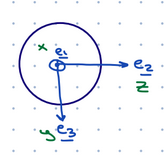
\includegraphics{Dawson-figures/coords-2.2.png}

For the body forces, we can first get an expression for the position-dependent density of the gel. The density gradient is linear in the $\bm{e_2}$ direction with $\rho(x_2 = -R) = \rho_w/2$ and $\rho(x_2 = R) = 3\rho_w/2$. We can use these two points to get a linear expression for the density.
\begin {equation}
    \rho(\bm{x}) = \frac{\rho_w}{2 R}x_2 + \rho_w
\end{equation}
The body forces on the gel are $\bm{b} = \rho \bm{g}$. Since $\bm{g}$ points downward, this means the overall body forces on the gel will be $\bm{b} = \rho g \bm{e_3} = (\frac{\rho_w}{2 R}x_2 + \rho_w)g \bm{e_3}$. This is using the coordinate system deified in the image and at the start of this problem, with $\bm{e_3}$ pointing downwards.
\begin{equation}
    \bm{F_b} =  \int_{\Omega}\bm{b} \space dV_{\bm{x}} =\int_{\Omega}  (\frac{\rho_w}{2 R}x_2 + \rho_w)g \bm{e_3} \space dV_{\bm{x}} = g \bm{e_3} \int_{\Omega}  (\frac{\rho_w}{2 R}x_2 + \rho_w) \space dV_{\bm{x}}
\end{equation}
To integrate, we use spherical coordinates. Using the definitions below (from Mathematical Methods in the Physical Sciences by Mary L. Boas, 3rd edition) and the assignment of a right-handed $xyz$ coordinate system stated at the start of the problem, this gives us $x_1 = r\sin{\theta}\cos{\phi}$, $x_2 = r\cos{\theta}$, and $x_3 = r\sin{\theta}\sin{\phi}$.

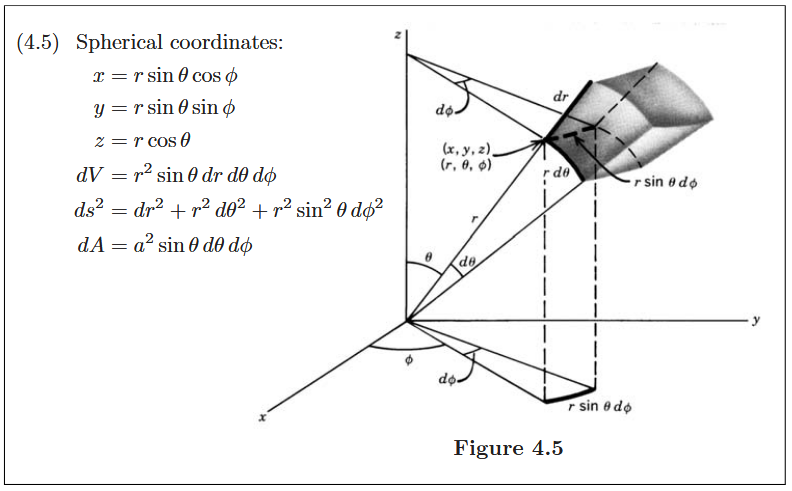
\includegraphics[scale=0.5]{Dawson-figures/boas-spherical.png}

We also use that $dV = r^2 \sin{\theta}drd\theta d\phi$ to put the volume integral into spherical.
\begin{equation}
    \bm{F_b}=g\bm{e_3} \int_{\Omega}  (\frac{\rho_w}{2 R}(r\cos{\theta}) + \rho_w) \space r^2 \sin{\theta} \space drd\theta d\phi
\end{equation}
We can then distribute over the sum and separate out the integral into two terms. We also pull out additional constants and note that the volume integral is really a triple integral over each of the three integration variables.
\begin{equation}
    \bm{F_b} = \bm{e_3}g \left[ \frac{\rho_w}{2 R} \int_{r} \int_{\theta} \int_{\phi}r^3 \cos{\theta}\sin{\theta} \space drd\theta d\phi + \rho_w\int_{r} \int_{\theta} \int_{\phi} r^2 \sin{\theta} \space drd\theta d\phi \right]
\end{equation}
Then we can integrate over the volume of the spherical gel, further separating out each of our independent variables for integration. Our bounds for integration are $r=0$ to $R$, $\theta=0$ to $\pi$, and $\phi = 0$ to $2\pi$.
\begin{equation}
    \bm{F_b} = \bm{e_3}g \left[ \frac{\rho_w}{2 R} \int_{0}^{R} r^3 dr\int_{0}^{\pi} \cos{\theta}\sin{\theta} \space d\theta\int_{0}^{2\pi} d\phi  + \rho_w\int_{0}^{R} r^2 dr\int_{0}^{\pi}\sin{\theta} \space d\theta\int_{0}^{2\pi} d\phi\right]
\end{equation}

\begin{equation}
    \bm{F_b} = \bm{e_3}g \left[ 0  + \rho_w \frac{R^3}{3}(2)(2\pi) \right] = \bm{e_3}g \left(\frac{4\pi}{3} \rho_w R^3 \right) = \frac{4}{3}\pi\rho_w g R^3 \bm{e_3}
\end{equation}

For the traction forces, we can first get an expression for the unit area vector $\bm{\hat{n}}$ of the sphere in cartesian coordinates. For our sphere, the unit normal $\bm{\hat{n}}$ points radially outward from the center of our shifted coordinate system and is at radial distance $R$ from the center of our coordinate system. This means we can write $\bm{\hat{n}}$ in the direction of our point from the center (simply the cartesian location) divided by radius $R$ (dividing by the magnitude to make this a unit vector), giving us the following expression for points on the surface of the gel.
\begin{equation}
    \bm{\hat{n}} = \frac{1}{R}(x_1\bm{e_1} + x_2\bm{e_2} + x_3\bm{e_3})
\end{equation}
From this, we can write the traction force specific to our problem in cartesian coordinates as $\bm{t} = -\rho_w g x_3 \hat{\bm{n}} = \frac{-\rho_w g x_3}{R}(x_1\bm{e_1} + x_2\bm{e_2} + x_3\bm{e_3})$ and put this into the integral for the total traction forces on the gel.
\begin{equation}
    \bm{F_t} = \int_{\partial \Omega_t}\bm{t} \space dA_{\bm{x}} = \int_{\partial \Omega_t} \frac{-\rho_w g}{R}x_3(x_1\bm{e_1} + x_2\bm{e_2} + x_3\bm{e_3}) \space dA_{\bm{x}}
\end{equation}
\begin{equation}
    \bm{F_t} = \frac{-\rho_w g}{R} \left[ \bm{e_1} \int_{\partial \Omega_t}x_3x_1 dA_{\bm{x}} + \bm{e_2} \int_{\partial \Omega_t}x_3x_2 dA_{\bm{x}} + \bm{e_3} \int_{\partial \Omega_t}x_3x_3 dA_{\bm{x}} \right]
\end{equation}
We can evaluate our integrals in spherical coordinates using the same assignments as for the body force integral, but using $dA = r^2 \sin{\theta}d\theta d\phi$ to put the surface integral into spherical.
\begin{equation}
\begin{split}
    \bm{F_t} = \frac{-\rho_w g}{R} \biggr[ \bm{e_1} \int_{\partial \Omega_t}r^4 \sin^3{\theta}\sin{\phi}\cos{\phi} \space d\theta d\phi  \\  + \bm{e_2} \int_{\partial \Omega_t} r^4 \sin^2{\theta}\cos{\theta}\sin{\phi} \space d\theta d\phi + \bm{e_3} \int_{\partial \Omega_t} r^4 \sin^3{\theta}\sin^2{\phi} \space d\theta d\phi \biggr]
\end{split}
\end{equation}
The integral is performed at the surface with $r=R$ and with bounds for integration $\theta=0$ to $\pi$ and $\phi = 0$ to $2\pi$.
\begin{equation}
\begin{split}
    \bm{F_t} = \frac{-\rho_w g R^4}{R} \biggr[ \bm{e_1} \int_{0}^{\pi} \sin^3{\theta} \space d\theta \int_{0}^{2\pi}\sin{\phi}\cos{\phi} \space d\phi \\
    + \bm{e_2} \int_{0}^{\pi} \sin^2{\theta}\cos{\theta} \space d\theta\int_{0}^{2 \pi}\sin{\phi} \space d\phi + \bm{e_3} \int_{0}^{\pi}\sin^3{\theta} \space d\theta \int_{0}^{2\pi} \sin^2{\phi} \space d\phi \biggr]
    \end{split}
\end{equation}
\begin{equation}
    \bm{F_t} = -\rho_w g R^3 \left[ \bm{e_1} (0) + \bm{e_2} (0) + \bm{e_3} (4/3)(\pi) \right] = -\frac{4}{3}\pi\rho_w g R^3 \bm{e_3}
\end{equation}
Summing the contributions from body and traction forces, we get a net force as follows.
\begin{equation}
    \bm{F_{net}} = \bm{F_{b}} + \bm{F_{t}} = \frac{4}{3}\pi\rho_w g R^3 \bm{e_3} -\frac{4}{3}\pi\rho_w g R^3 \bm{e_3} = \bm{0}
\end{equation}
\hspace*{\fill} $\bigstar$

Net moment on the gel is from both the traction forces $\bm{M_t}$ and body forces $\bm{M_b}$. The same simplified coordinate system will be used in calculating the net moment as was used for the net force, defined at the start.
\begin{equation}
    \bm{M_b} = \int_{\Omega}\bm{x} \times \bm{b} \space dV_{\bm{x}} \space ; \space \bm{M_t} = \int_{\partial \Omega_t} \bm{x} \times \bm{t} \space dA_{\bm{x}}
\end{equation}
For the body moment, we first perform the cross product with $\bm{b} = \rho g \bm{e_3}$ and $\bm{x} = x_1 \bm{e_1} + x_2 \bm{e_2} + x_3 \bm{e_3}$.
\begin{equation}
    \bm{x} \times \bm{b} = \rho g x_2 \bm{e_1} - \rho g x_1 \bm{e_2} = \rho g (x_2\bm{e_1} - x_1 \bm{e_2})
\end{equation}
This cross product then goes into the integral for the body moment.
\begin{equation}
    \bm{M_b} = \int_{\Omega}\bm{x} \times \bm{b} \space dV_{\bm{x}} = \int_{\Omega} (\rho g)(x_2\bm{e_1} - x_1 \bm{e_2}) dV_{\bm{x}} = \bm{e_1}\int_{\Omega} \rho gx_2dV_{\bm{x}} - \bm{e_2}\int_{\Omega} \rho gx_1 dV_{\bm{x}}
\end{equation}
Then we can sub in our expression for density $\rho(\bm{x}) = (\rho_w/2 R)x_2 + \rho_w$ and convert our integrals to spherical.
\begin{equation}
    \bm{M_b} = \bm{e_1}g \int_{\Omega} (\frac{\rho_w}{2R}x_2 + \rho_w) x_2dV_{\bm{x}} - \bm{e_2}g\int_{\Omega} (\frac{\rho_w}{2R}x_2 + \rho_w)x_1 dV_{\bm{x}}
\end{equation}
\begin{equation}
\begin{split}
    \bm{M_b} = \bm{e_1}g \left[ \int_{\Omega} \frac{\rho_w}{2R}x_2x_2dV_{\bm{x}} + \int_{\Omega}\rho_w x_2dV_{\bm{x}} \right] \\
    - \bm{e_2}g \left[ \int_{\Omega} \frac{\rho_w}{2R}x_2x_1 dV_{\bm{x}} + \int_{\Omega}\rho_w x_1dV_{\bm{x}}\right]
\end{split}
\end{equation}

\begin{equation}
\begin{split}
    \bm{M_b} = \bm{e_1}g \left[ \frac{\rho_w}{2R}\int_{\Omega}r^4\cos^2{\theta} \sin{\theta}drd\theta d\phi + \rho_w \int_{\Omega}r^3\cos{\theta}\sin{\theta}drd\theta d\phi \right] \\
    - \bm{e_2}g \left[ \frac{\rho_w}{2R}\int_{\Omega} r^4 \sin^2{\theta}\cos{\theta}\cos{\phi}drd\theta d\phi + \rho_w\int_{\Omega} r^3\sin^2{\theta}\cos{\phi}drd\theta d\phi \right]
\end{split}
\end{equation}
Perform the integral with bounds $r=0$ to $R$, $\theta=0$ to $\pi$, and $\phi = 0$ to $2\pi$.
\begin{equation}
\begin{split}
    \bm{M_b} = \bm{e_1}g \left[ \frac{\rho_w}{2R}\int_{0}^{R}r^4 dr \int_{0}^{\pi}\cos^2{\theta} \sin{\theta} \space d\theta \int_{0}^{2\pi}d\phi + \rho_w \int_{0}^{R}r^3dr \int_{0}^{\pi}\cos{\theta}\sin{\theta} \space d\theta \int_{0}^{2\pi}d\phi \right] \\
    - \bm{e_2}g \left[ \frac{\rho_w}{2R}\int_{0}^{R}r^4dr \int_{0}^{\pi}\sin^2{\theta}\cos{\theta} \space d\theta \int_{0}^{2\pi}\cos{\phi}\space d\phi + \rho_w\int_{0}^{R}r^3 dr\int_{0}^{\pi}\sin^2{\theta} \space d\theta \int_{0}^{2\pi}\cos{\phi} \space d\phi \right]
\end{split}
\end{equation}
\begin{equation}
    \bm{M_b} = \bm{e_1}g \left[ \frac{\rho_w}{2R} (R^5/5)(2/3)(2\pi) + \rho_w (R^4/4)(0)(2\pi) \right] - \bm{e_2}g \left[ \frac{\rho_w}{2R}(0) + \rho_w (0) \right]
\end{equation}
\begin{equation}
    \bm{M_b} = \bm{e_1}g \left[ \frac{\rho_w}{2R} (R^5/5)(2/3)(2\pi)\right] = \frac{2\pi}{15}R^4\rho_w g \bm{e_1}
\end{equation}

For the traction moment, we first perform the cross product with $\bm{t} = \frac{-\rho_w g x_3}{R}(x_1\bm{e_1} + x_2\bm{e_2} + x_3\bm{e_3})$ and $\bm{x} = x_1 \bm{e_1} + x_2 \bm{e_2} + x_3 \bm{e_3}$.
\begin{equation}
    \bm{x} \times \bm{t} = 0 \bm{e_1} + 0 \bm{e_2} + 0 \bm{e_3} = \bm{0}
\end{equation}
This cross product then goes into the integral for the body moment.
\begin{equation}
    \bm{M_t} = \int_{\Omega}\bm{x} \times \bm{t} \space dV_{\bm{x}} = \int_{\Omega} \bm{0} \space dV_{\bm{x}} = \bm{0}
\end{equation}
Summing the contributions from body and traction moment, we get a net moment as follows.
\begin{equation}
    \bm{M_{net}} = \bm{M_{b}} + \bm{M_{t}} = \frac{2\pi}{15}R^4\rho_w g \bm{e_1} + \bm{0} = \frac{2\pi}{15}R^4\rho_w g \bm{e_1}
\end{equation}
\hspace*{\fill} $\bigstar$
\medskip

(b) $\mathcal{B}$ is in static equilibrium when:

(1) The average density of the gel matches that of water (or more generally, the density of the fluid the gel in submerged in). This would establish a net force of zero, and is true for the current configuration of the gel sphere in water with the problem-defined density gradient.

(2) The center of mass established by the density gradient is aligned with the center of volume of the sphere. That is, if we were to rotate the sphere so that the density gradient is along the $\bm{e_3}$ axis, the net body force would act along that axis and in line with the center of our coordinate system (and the center of volume where the buoyant force effectively acts) and therefore not contribute to the net moment. This would establish a net moment of zero, and is not true for the current configuration of the gel sphere in water.

\bigskip
\subsection*{2--3. \textbf{Viscoelastic data}} 

\medskip
(a) For linear viscoelasticity, isochrones should be linear. This material cannot be fully described with LVE, but the assumption should be valid in the roughly linear region for for strain $\varepsilon = 0$ to about $2 \times 10^-3$ and stress $\sigma = 0$ to about 300 Pa.

\medskip
(b) We expect the strain response for a step stress $\sigma(t) = \sigma_0 H(t)$ to be $\varepsilon(t) = J_c(t,\sigma)\sigma_0$. To get $J_c(t)$ for a given stress, we can estimate the strain function $\varepsilon(t)$ at that stress value and use this relationship to get the following for a given $\sigma_0$ value.
\begin{equation}
    \varepsilon(t) = J_c(t)\sigma_0 \to J_c(t) = \frac{1}{\sigma_0} \varepsilon(t)
\end{equation}

For 100Pa, we look at the the strain values for each time along that stress value. Looking along the $\sigma = 100$Pa line, we estimate $\varepsilon(2) = 0.44 \times 10^{-3}$, $\varepsilon(5) = 0.54 \times 10^{-3}$, $\varepsilon(10) = 0.67 \times 10^{-3}$, $\varepsilon(20) = 0.82 \times 10^{-3}$, $\varepsilon(40) = 0.99 \times 10^{-3}$. Plotting these values we get the following.

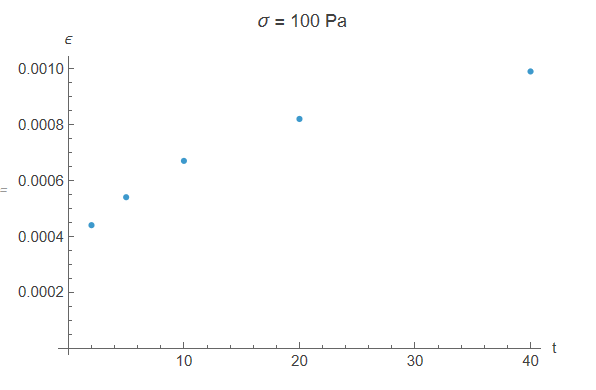
\includegraphics[scale=0.5]{Dawson-figures/100-data.png}

Visually, this plot looks like it could be a logarithmic or square root fit for $\varepsilon(t)$. This would suggest a form of $\varepsilon(t) = A\ln{t}+B$ or $\varepsilon(t) = A\sqrt{t}+B$. To test, we make plots of $\varepsilon$ vs $\ln{t}$ and $\sqrt{t}$ and a linear fit to this data.

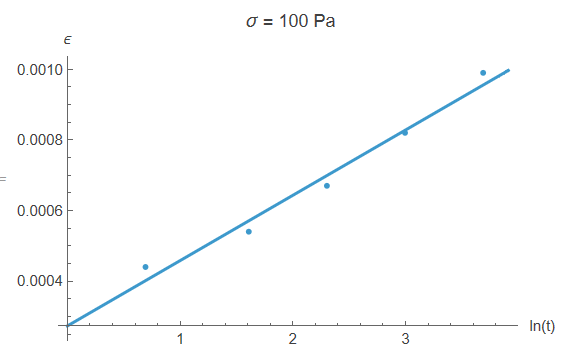
\includegraphics[scale=0.5]{Dawson-figures/100-ln.png}
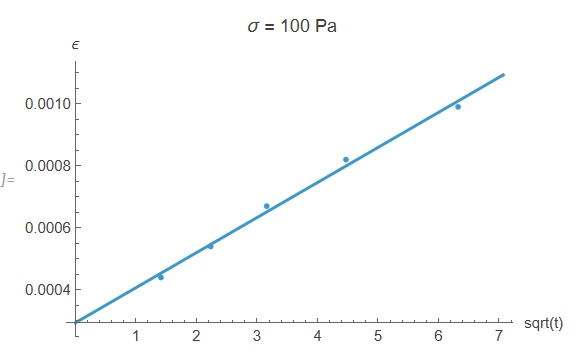
\includegraphics[scale=0.5]{Dawson-figures/100-sqrt.png}

Looking at these plots, it seems that $\varepsilon(t) = A\sqrt{t}+B$ will be a better fit to this data. We use the linear fit of $y = (1.13 \times10^{-4})x + (2.94 \times 10^{-4})$ to get a corresponding expression for $\varepsilon(t)$. 
\begin{equation}
    \varepsilon(t) =(1.13 \times10^{-4})\sqrt{t}+(2.94 \times 10^{-4})
\end{equation}
Which we can plot and see that it estimates our data reasonably well.

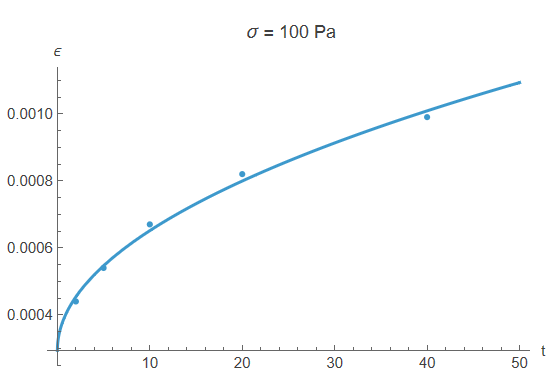
\includegraphics[scale=0.5]{Dawson-figures/100-full.png}

Then, dividing by the constant stress values $\sigma_0 = 100$ Pa, we can get a relationship for $J_c(t)$.
\begin{equation}
    J_c(t) =(1.13 \times10^{-6})\sqrt{t}+(2.94 \times 10^{-6})
\end{equation}
\hspace*{\fill} $\bigstar$
\medskip

We can then repeat a similar process for 250Pa. Looking along the $\sigma = 250$Pa line, we estimate $\varepsilon(2) = 1.2 \times 10^{-3}$, $\varepsilon(5) = 1.45 \times 10^{-3}$, $\varepsilon(10) = 1.80 \times 10^{-3}$, $\varepsilon(20) = 2.40 \times 10^{-3}$, $\varepsilon(40) = 3.00 \times 10^{-3}$. Plotting these values we get the following.

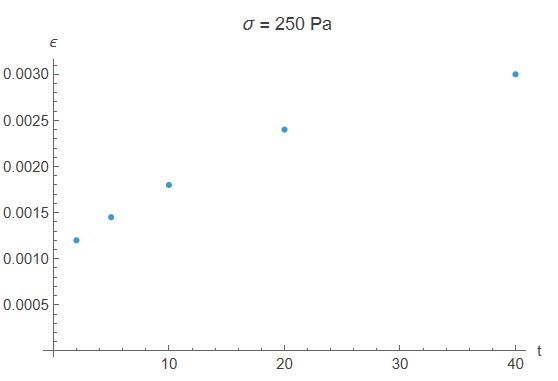
\includegraphics[scale=0.5]{Dawson-figures/250-data.png}

Repeating the same plots of $\varepsilon$ vs $\ln{t}$ and $\sqrt{t}$ and linearly fitting the data, we once again see that an expression of the form $\varepsilon(t) = A\sqrt{t}+B$ will likely estimate the data well.

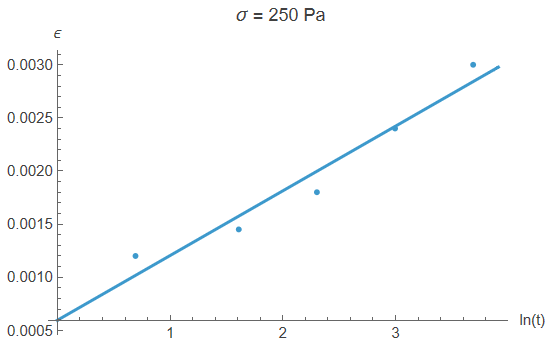
\includegraphics[scale=0.5]{Dawson-figures/250-ln.png}
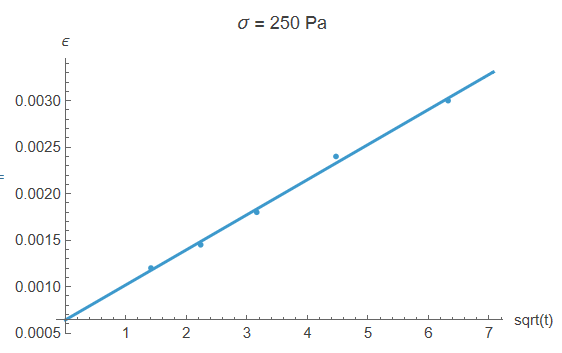
\includegraphics[scale=0.5]{Dawson-figures/250-sqrt.png}

From the linear fit of $y = (1.13 \times10^{-4})x + (2.94 \times 10^{-4})$ we can get an expression for $\varepsilon(t)$.
\begin{equation}
    \varepsilon(t) =(3.77 \times10^{-4})\sqrt{t}+(6.42 \times 10^{-4})
\end{equation}
Plotting this relationship with the estimated $\varepsilon(t)$ data points we can see a reasonably good fit as well.

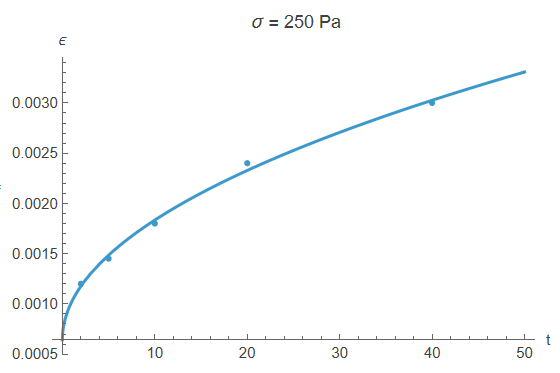
\includegraphics[scale=0.5]{Dawson-figures/250-full.png}

Dividing by the constant stress value $\sigma_0 = 250$ Pa, we can get a relationship for $J_c(t)$.
\begin{equation}
    J_c(t) =(1.508 \times10^{-6})\sqrt{t}+(2.568 \times 10^{-6})
\end{equation}
\hspace*{\fill} $\bigstar$

\bigskip
\subsection*{2--4. \textbf{Impulsive stresses}}
\medskip
(a) For LVE we can use superposition to combine step load responses into responses to an arbitrary stress function according to the following relationship.
\begin{equation}
    \varepsilon(t) = \int_{0}^{t}J_c(t-\tau)\frac{d\sigma(\tau)}{d\tau}d\tau
\end{equation}
We can solve this relationship for the given stress function of $\sigma(t) = A \delta(t)$ using a Laplace transformation. We take the Laplace transform of both sides of the above expression, noting that the expression is a convolution of two functions to a product of two Laplace transforms.
\begin{equation}
    \mathcal{L}\{ \varepsilon(t)\} = \mathcal{L}\{ \int_{0}^{t}J_c(t-\tau)\frac{d\sigma(\tau)}{d\tau}d\tau\} = \mathcal{L}\{ J_c(t)\}\mathcal{L}\{ \frac{d \sigma(t)}{d t}\}
\end{equation}
Subbing in our stress function $\sigma(t) = A \delta(t)$ we get the Laplace transform of $J_c(t)$ and of the derivative of $\delta(t)$.
\begin{equation}
    \mathcal{L}\{ \varepsilon(t)\} = \mathcal{L}\{ J_c(t)\}\mathcal{L}\{ \frac{d}{d t} A \delta(t)\} = A \overline{J_c}(s)\mathcal{L}\{ \frac{d}{d t}\delta(t)\}
\end{equation}
We note that $\mathcal{L}\{ \delta(t) \} = 1$, $\mathcal{L}\{ \delta^{(1)}(t) \} = s$, $\mathcal{L}\{ \delta^{(2)}(t) \} = s^2$, and so on such that the nth derivative of $\delta(t)$ has a Laplace transform $\mathcal{L}\{ \delta^{(n)}(t) \} = s^n$. Therefore, we can take the Laplace transform of $\mathcal{L}\{ \frac{\partial}{\partial t} \delta(t) \} = s$.
\begin{equation}
    \mathcal{L}\{ \varepsilon(t)\} = A s \overline{J_c}(s)
\end{equation}
Then we can take the inverse Laplace transform of both sides, where we note that $\mathcal{L} \{ \frac{d}{dt} f(t) \} = sF(s) - f(0)$ giving us an inverse Laplace transform of $ \frac{d}{dt} f(t) = \mathcal{L}^{-1} \{ sF(s) - f(0) \}$. Also note that $\mathcal{L}\{ \delta(t) \} = 1$ so that $\mathcal{L}^{-1} \{ 1 \} = \delta(t)$ and $\mathcal{L}^{-1} \{ C \} = C\delta(t)$.
\begin{equation}
    \varepsilon(t) = \mathcal{L}^{-1}\{ A s \overline{J_c}(s) \} = A \mathcal{L}^{-1}\{s \overline{J_c}(s)  - J_c(0) + J_c(0)\}
\end{equation}
\begin{equation}
    \varepsilon(t) = A \mathcal{L}^{-1}\{s \overline{J_c}(s)  - J_c(0) \} + A\mathcal{L}^{-1} \{J_c(0)\}
\end{equation}
Taking the inverse Laplace transform of both of these pieces we get the following for the general creep relaxation function.
\begin{equation}
    \varepsilon(t) = A \frac{d}{dt}J_c(t) + AJ_c(0)\delta(t)
\end{equation}
\hspace*{\fill} $\bigstar$
\medskip

For the Kelvin-Voigt model, we can use the expression for the response of a Kelvin-Voigt solid to an arbitrary stress.
\begin{equation}
    \varepsilon(t) = \frac{\sigma(t = 0^-)}{E}(1-\exp[-Et/\eta]) + \frac{1}{E} \int_{0^-}^{t}(1 - \exp[\frac{-E(t-\tau)}{\eta}]\frac{d\sigma(\tau)}{d\tau}d\tau
\end{equation}
For the stress function $\sigma(t) = A \delta(t)$, $\sigma(0^-) = 0$ so the first term goes away to zero. Then we take a Laplace transform of both sides to solve for $\varepsilon(t)$.
\begin{equation}
    \mathcal{L}\{ \varepsilon(t)\} = \frac{1}{E}\mathcal{L}\{  \int_{0^-}^{t}(1 - \exp[\frac{-E(t-\tau)}{\eta}]\frac{d\sigma(\tau)}{d\tau}d\tau \}
\end{equation}
We once again note that this is the Laplace transform of a convolution, which is equal to the product of the Laplace transform for the two component functions of the convolution.
\begin{equation}
    \mathcal{L}\{ \varepsilon(t)\} = \frac{1}{E}\mathcal{L}\{1 - \exp[\frac{-Et}{\eta}]\} \mathcal{L}\{\frac{d\sigma(t)}{dt}\} = \frac{1}{E}\mathcal{L}\{1 - \exp[\frac{-Et}{\eta}]\} \mathcal{L}\{\frac{d}{dt} A\delta(t)\}
\end{equation}
Taking the Laplace transforms, noting that $\mathcal{L}\{\frac{d}{dt}\delta(t) \} =  s$, $\mathcal{L}\{e^{-at} \} = \frac{1}{s+a}$, and $\mathcal{L}\{1\} =1/s$.
\begin{equation}
    \mathcal{L}\{ \varepsilon(t)\} = \frac{A}{E}(\frac{1}{s}-\frac{1}{s+E/\eta})(s) = \frac{A}{E}(1 - \frac{s}{s+E/\eta})
\end{equation}
\begin{equation}
    \mathcal{L}\{ \varepsilon(t)\} = \frac{A}{E}- \frac{A}{E}\frac{s + E/\eta - E/\eta}{s+E/\eta} = \frac{A}{E}- \frac{A}{E}(1-\frac{E/\eta}{s+E/\eta})
\end{equation}
\begin{equation}
    \mathcal{L}\{ \varepsilon(t)\} = \frac{A}{\eta}(\frac{1}{s+E/\eta})
\end{equation}
Then doing the inverse Laplace transform of both sides and noting $\mathcal{L}^{-1}\{\frac{1}{s + a}\} = e^{-at}$ we get the following for the Kelvin-Voigt model.
\begin{equation}
    \varepsilon(t) = \frac{A}{\eta}e^{-Et/\eta}
\end{equation}
\hspace*{\fill} $\bigstar$
\medskip \newline
We could also get this result by subbing $J_c(t)$ for the Kelvin-Voigt model into our expression with this stress function for a general creep relaxation function.

(b) We repeat a similar process for the stress function $\sigma(t) = B \psi(t) = B \frac{d}{dt}\delta(t)$. Starting from the strain function for a general stress function and taking the Laplace transformation.
\begin{equation}
    \varepsilon(t) = \int_{0}^{t}J_c(t-\tau)\frac{d\sigma(\tau)}{d\tau}d\tau
\end{equation}
\begin{equation}
    \mathcal{L}\{ \varepsilon(t)\} = \mathcal{L}\{ J_c(t)\}\mathcal{L}\{ \frac{d \sigma(t)}{d t}\} = \overline{J_c}(s) \mathcal{L}\{ B\delta^{(2)}(t) \}
\end{equation}
We note that $\mathcal{L}\{ \delta^{(2)}(t) \} = s^2$.
\begin{equation}
    \mathcal{L}\{ \varepsilon(t)\} = \overline{J_c}(s) B s^2
\end{equation}
Then taking the inverse Laplace transform and noting that both $\mathcal{L} \{ \frac{d}{dt} f(t) \} = sF(s) - f(0)$ giving us an inverse Laplace transform of $ \frac{d}{dt} f(t) = \mathcal{L}^{-1} \{ sF(s) - f(0) \}$ and $\mathcal{L} \{ \frac{d^2}{dt^2} f(t) \} = s^2F(s) - sf(0) - f'(0)$ giving us an inverse Laplace transform $ \frac{d^2}{dt^2} f(t) = s^2F(s) - sf(0) - f'(0)$. We also note that $\mathcal{L}\{ \delta(t) \} = 1$ and $\mathcal{L}\{ \delta'(t) \} = s$ so that $\mathcal{L}^{-1}\{ 1 \} = \delta(t)$ and $\mathcal{L}^{-1}\{ s \} = \delta'(t)$.
\begin{equation}
    \varepsilon(t) = \mathcal{L}^{-1}\{ \overline{J_c}(s) B s^2 \} = B\mathcal{L}^{-1}\{ s^2\overline{J_c}(s) \}
\end{equation}
\begin{equation}
    \varepsilon(t) = B\mathcal{L}^{-1}\{ s^2\overline{J_c}(s)  - sJ_c(0) - \dot{J_c}(0)\} + B\mathcal{L}^{-1}\{ sJ_c(0)\} + B\mathcal{L}^{-1}\{ \dot{J_c}(0)\}
\end{equation}
Doing so, we get the following expression for a general creep relaxation function.
\begin{equation}
    \varepsilon(t) = B\frac{d^2}{dt^2}J_c(t) + B\dot{J_c}(0)\delta(t) + BJ_c(0)\delta'(t)
\end{equation}
\hspace*{\fill} $\bigstar$
\medskip

For the Kelvin-Voigt model we start from the same expression for an arbitrary stress on the Kelvin-Voigt model as we did in part (a).
\begin{equation}
    \varepsilon(t) = \frac{\sigma(t = 0^-)}{E}(1-\exp[-Et/\eta]) + \frac{1}{E} \int_{0^-}^{t}(1 - \exp[\frac{-E(t-\tau)}{\eta}]\frac{d\sigma(\tau)}{d\tau}d\tau
\end{equation}
Note that $\sigma(0^-)=0$ so the first term goes away. We then take the Laplace transform .
\begin{equation}
    \mathcal{L}\{ \varepsilon(t)\} =  \frac{B}{E}\mathcal{L}\{1 - \exp[\frac{-Et}{\eta}]\} \mathcal{L}\{\frac{d}{dt}\frac{d}{dt}\delta(t)\} = \frac{B}{E}s^2(\frac{1}{s} - \frac{1}{s + E/\eta})
\end{equation}
\begin{equation}
    \mathcal{L}\{ \varepsilon(t)\} = \frac{B}{E}(s - \frac{s^2}{s + E/\eta}) =  \frac{Bs}{E} - \frac{B}{E}(\frac{s^2}{s+a})
\end{equation}
Then we can take the inverse Laplace transform, and get the strain for the Kelvin-Voigt model as follows.
\begin{equation}
    \varepsilon(t) = \frac{B}{E}\delta'(t) - \frac{B}{E} \left[ \delta'(t)+\frac{E^2}{\eta^2}e^{-Et/\eta}- \frac{E}{\eta}\delta(t) \right]
\end{equation}
\begin{equation}
    \varepsilon(t) = \frac{-EB}{\eta^2}e^{-Et/\eta} + \frac{B}{\eta}\delta(t)
\end{equation}
\hspace*{\fill} $\bigstar$
\medskip


\bigskip
\subsection*{2--5. \textbf{Two-element models}}
(a) The constitutive law for the Kelvin-Voigt model is $\eta \dot{\varepsilon} + E\varepsilon = \sigma(t)$. For this deformation, the initial strain at $t=0$ is $\varepsilon(0) = -d/h$ (since $\varepsilon=\Delta L/L$). Then the strain oscillates between $-2d$ and $0$.
\begin{equation}
    \varepsilon(t) = \frac{-d}{h} - \frac{d}{h}\sin{\omega t}
\end{equation}
\begin{equation}
    \dot{\varepsilon}(t) = \frac{-d \omega}{h}\cos{\omega t}
\end{equation}
Putting this strain into the constitutive equation.
\begin{equation}
    \sigma(t) = \eta \dot{\varepsilon} + E\varepsilon = \frac{-\eta \omega d}{h}\cos{\omega t} + E(\frac{-d}{h} - \frac{d}{h}\sin{\omega t})
\end{equation}
\begin{equation}
    \sigma(t) = \frac{-\eta \omega d}{h}\cos{\omega t} + \frac{-Ed}{h} - \frac{Ed}{h}\sin{\omega t}
\end{equation}
\hspace*{\fill} $\bigstar$
\medskip

(b) Strain is applied at $\sin{\omega t}$. To get the difference in phase (or phase lag) for the stress we can combine the expression we got in part (a) to a single sine term so that we can get the oscillations in the form $\sin{(\omega t + \delta)}$. We first use $\cos{\omega t} = \sin{(\omega t + \pi/2)}$.
\begin{equation}
    \sigma(t) = \frac{-\eta \omega d}{h}\sin{(\omega t + \pi/2)} + \frac{-Ed}{h} - \frac{Ed}{h}\sin{\omega t}
\end{equation}
To add two sine functions we note that for $E_1 + E_2 = E_3$ with $E_1 = E_{10}\sin{\omega t}$ and $E_2 = E_{20}\sin{(\omega t + \Delta)}$ we get $E_3 = E_{30}\sin{(\omega t + \phi)}$ with $E_{30} = \sqrt{E^2_{10} + E^2_{20} + 2E_{10}E_{20}\cos{\Delta}}$ and $\tan{\phi} = \frac{E_{20}\sin{\Delta}}{E_{10}+E_{20}\cos{\Delta}}$. Using these expressions we can get the stress function into a single sine function with a phase lag as follows below.
\begin{equation}
    \tan{\phi} = \tan{\delta} = \frac{(-\eta\omega d/h)\sin{\pi/2}}{(-Ed/h) + (-\eta\omega d/h)\cos{\pi/2}} = \frac{\eta\omega}{E}
\end{equation}
\hspace*{\fill} $\bigstar$
\medskip

(c) Given the stress we can determine the strain also by solving the differential equation for the constitutive law for a Kelvin-Voigt material.
\begin{equation}
    \sigma(t) = \eta \dot{\varepsilon} + E\varepsilon = -\sigma_0 - \sigma_0\sin{\omega t}
\end{equation}
Solving the differential equation for strain $\varepsilon(t)$ in Mathematica we get the following.
\begin{equation}
    \varepsilon(t) = Ce^{-Et/\eta} - \frac{\sigma_0}{E^3 + \omega^2 \eta^2E}(E^2 + \omega^2 \eta^2 - \omega E \eta \cos{\omega t} + E^2 \sin{\omega t})
\end{equation}
Using initial condition $\varepsilon(0) = \varepsilon_0 = -d/h$ we get the following.
\begin{equation}
    \varepsilon(0) = C - \frac{\sigma_0}{E^3 + \omega^2 \eta^2E}(E^2 + \omega^2 \eta^2 - \omega E \eta (1) + E^2 (0)) = \varepsilon_0
\end{equation}
\begin{equation}
    C = \varepsilon_0 +  \frac{\sigma_0}{E(E^2 + \omega^2 \eta^2)}(E^2 + \omega^2 \eta^2 - \omega\eta E) = \frac{d}{h} +  \frac{\sigma_0}{E(E^2 + \omega^2 \eta^2)}(E^2 + \omega^2 \eta^2 - \omega\eta E)
\end{equation}
We can sub this in for our constant to get a final expression for $\varepsilon(t)$.
\begin{equation}
     \varepsilon(t) =\left[ \frac{d}{h} +  \frac{\sigma_0 (E^2 + \omega^2 \eta^2 - \omega\eta E)}{E(E^2 + \omega^2 \eta^2)}\right]  e^{-Et/\eta} - \frac{\sigma_0}{E(E^2 + \omega^2 \eta^2)}(E^2 + \omega^2 \eta^2 - \omega E \eta \cos{\omega t} + E^2 \sin{\omega t})
\end{equation}
\hspace*{\fill} $\bigstar$
\medskip

(d) We can look at the above expression at larger times, where the contribution of the exponential term will decrease and the behavior is mainly sinusoidal. Doing so, we can look at combining our terms into a single sine function (or at least find the phase difference for that combined sine function from the stress input) to see what the phase lag would be for the sinusoidal part of the material response. Note that the frequency for the stress is related to $\sin{\omega t}$ this time, and we will directly find the phase difference for the strain.

For large times we can simplify the expression from part (c) to ignore the exponential term.
\begin{equation}
     \varepsilon(t) \approx \frac{-\sigma_0}{E(E^2 + \omega^2 \eta^2)}(E^2 + \omega^2 \eta^2 - \omega E \eta \cos{\omega t} + E^2 \sin{\omega t})
\end{equation}
We first use $\cos{\omega t} = \sin{(\omega t + \pi/2)}$.
\begin{equation}
     \varepsilon(t) \approx \frac{-\sigma_0}{E(E^2 + \omega^2 \eta^2)}(E^2 + \omega^2 \eta^2 - \omega E \eta \sin{(\omega t +\pi/2)} + E^2 \sin{\omega t})
\end{equation}
\begin{equation}
     \varepsilon(t) \approx \frac{-\sigma_0}{E(E^2 + \omega^2 \eta^2)}(E^2 + \omega^2 \eta^2) + \frac{\sigma_0 \omega\eta}{(E^2 + \omega^2 \eta^2)} \sin{(\omega t +\pi/2)} + \frac{-\sigma_0 E}{(E^2 + \omega^2 \eta^2)} \sin{\omega t}
\end{equation}
Then for the sum of the sine terms, we get $\tan{\phi}$ of the combined function $E_{30}\sin{\omega t + \phi}$ based on the same formulas used in part (b).
\begin{equation}
    \tan{\phi} = \frac{(\frac{\sigma_0 \omega\eta}{E^2 + \omega^2 \eta^2})\sin{\pi/2}}{(\frac{-\sigma_0 E}{E^2 + \omega^2 \eta^2}) + (\frac{\sigma_0 \omega\eta}{E^2 + \omega^2 \eta^2})\cos{\pi/2}} = \frac{\frac{\sigma_0 \omega\eta}{E^2 + \omega^2 \eta^2}}{\frac{-\sigma_0 E}{E^2 + \omega^2 \eta^2}} = \frac{-\omega \eta}{E}
\end{equation}
Once again, this is the phase difference for the strain function compared to the stress function. To get the phase lag of the stress behind the strain, we just invert the sign.
\begin{equation}
    \tan{\delta} = -\tan{\phi} = \frac{\omega \eta}{E}
\end{equation}
Which is the same as the phase lag found in part (b).
\hspace*{\fill} $\bigstar$


\end{document}